% eLife derivative manuscript template
%DIF LATEXDIFF DIFFERENCE FILE
%DIF DEL original/main.tex           Mon Feb 28 05:02:38 2022
%DIF ADD revision_1_eLife/main.tex   Mon Feb 28 06:11:04 2022
%%% PREAMBLE 
\documentclass[9pt]{elife}

\usepackage{bm}
\usepackage{caption}
\usepackage{float}
\usepackage{listings}
\usepackage{multirow}
\usepackage{siunitx}
\usepackage{subcaption}
\usepackage{soul}
\usepackage{adjustbox}
\usepackage{hyperref}
\usepackage{academicons}


\graphicspath{ {./Figures/} }

\setlength{\marginparwidth}{2cm}

%%%%%%%%%%%%%%%%%%%%%%%%%%%%%%%%%%%%%%%%%%%%%%%%%%%%%%%%%%%%
%%% ARTICLE SETUP
%%%%%%%%%%%%%%%%%%%%%%%%%%%%%%%%%%%%%%%%%%%%%%%%%%%%%%%%%%%%
\title{Identifying signatures of proteolytic stability and monomeric propensity in \emph{O}-glycosylated insulin using molecular simulation}

\author[1]{Wei-Tse Hsu} % ORCID: 0000-0001-6167-5480
\author[2]{Dominique A. Ramirez} % ORCID: 0000-0002-2944-8250
\author[3]{Tarek Sammakia} % ORCID: 0000-0003-3703-5672
\author[4]{Zhongping Tan}  % ORCID: 0000-0002-9302-150X
\author[1]{Michael R. Shirts} % ORCID: 0000-0003-3249-1097

\affil[1]{Department of Chemical \& Biological Engineering, University of Colorado Boulder, Boulder, CO, USA 80309}
\affil[2]{Department of Biochemistry, University of Colorado Boulder, Boulder, CO, USA 80309}
\affil[3]{Department of Chemistry, University of Colorado Boulder, Boulder, CO, USA 80309}
\affil[4]{Institute of Materia Medica, Chinese Academy of Medical Sciences, Peking Union Medical College, Beijing, 100050, China}

\corr{michael.shirts@colorado.edu}{MRS}
\corr{zhongping.tan@imm.pumc.edu.cn}{ZT}


%%%%%%%%%%%%%%%%%%%%%%%%%%%%%%%%%%%%%%%%%%%%%%%%%%%%%%%%%%%%
%%% ARTICLE START
%%%%%%%%%%%%%%%%%%%%%%%%%%%%%%%%%%%%%%%%%%%%%%%%%%%%%%%%%%%%
%DIF PREAMBLE EXTENSION ADDED BY LATEXDIFF
%DIF UNDERLINE PREAMBLE %DIF PREAMBLE
\RequirePackage[normalem]{ulem} %DIF PREAMBLE
\RequirePackage{color}\definecolor{RED}{rgb}{1,0,0}\definecolor{BLUE}{rgb}{0,0,1} %DIF PREAMBLE
\providecommand{\DIFaddtex}[1]{{\protect\color{blue}\uwave{#1}}} %DIF PREAMBLE
\providecommand{\DIFdeltex}[1]{{\protect\color{red}\sout{#1}}}                      %DIF PREAMBLE
%DIF SAFE PREAMBLE %DIF PREAMBLE
\providecommand{\DIFaddbegin}{} %DIF PREAMBLE
\providecommand{\DIFaddend}{} %DIF PREAMBLE
\providecommand{\DIFdelbegin}{} %DIF PREAMBLE
\providecommand{\DIFdelend}{} %DIF PREAMBLE
\providecommand{\DIFmodbegin}{} %DIF PREAMBLE
\providecommand{\DIFmodend}{} %DIF PREAMBLE
%DIF FLOATSAFE PREAMBLE %DIF PREAMBLE
\providecommand{\DIFaddFL}[1]{\DIFadd{#1}} %DIF PREAMBLE
\providecommand{\DIFdelFL}[1]{\DIFdel{#1}} %DIF PREAMBLE
\providecommand{\DIFaddbeginFL}{} %DIF PREAMBLE
\providecommand{\DIFaddendFL}{} %DIF PREAMBLE
\providecommand{\DIFdelbeginFL}{} %DIF PREAMBLE
\providecommand{\DIFdelendFL}{} %DIF PREAMBLE
%DIF HYPERREF PREAMBLE %DIF PREAMBLE
\providecommand{\DIFadd}[1]{\texorpdfstring{\DIFaddtex{#1}}{#1}} %DIF PREAMBLE
\providecommand{\DIFdel}[1]{\texorpdfstring{\DIFdeltex{#1}}{}} %DIF PREAMBLE
%DIF LISTINGS PREAMBLE %DIF PREAMBLE
\RequirePackage{listings} %DIF PREAMBLE
\RequirePackage{color} %DIF PREAMBLE
\lstdefinelanguage{DIFcode}{ %DIF PREAMBLE
%DIF DIFCODE_UNDERLINE %DIF PREAMBLE
  moredelim=[il][\color{red}\sout]{\%DIF\ <\ }, %DIF PREAMBLE
  moredelim=[il][\color{blue}\uwave]{\%DIF\ >\ } %DIF PREAMBLE
} %DIF PREAMBLE
\lstdefinestyle{DIFverbatimstyle}{ %DIF PREAMBLE
	language=DIFcode, %DIF PREAMBLE
	basicstyle=\ttfamily, %DIF PREAMBLE
	columns=fullflexible, %DIF PREAMBLE
	keepspaces=true %DIF PREAMBLE
} %DIF PREAMBLE
\lstnewenvironment{DIFverbatim}{\lstset{style=DIFverbatimstyle}}{} %DIF PREAMBLE
\lstnewenvironment{DIFverbatim*}{\lstset{style=DIFverbatimstyle,showspaces=true}}{} %DIF PREAMBLE
%DIF END PREAMBLE EXTENSION ADDED BY LATEXDIFF

\begin{document}

\maketitle

\begin{abstract}
Insulin has been commonly adopted as a peptide drug to treat diabetes given its ability to facilitate the uptake of glucose from the blood. The development of oral insulin remains elusive over decades owing to its susceptibility to the enzymes in the gastrointestinal tract and poor permeability through the intestinal epithelium upon dimerization. Recent experimental studies have revealed that certain \emph{O}-linked glycosylation patterns could enhance insulin's proteolytic stability and reduce its dimerization propensity, but the understanding of such phenomena at the molecular level is still evasive. To address this challenge, we \DIFdelbegin \DIFdel{propose and test }\DIFdelend \DIFaddbegin \DIFadd{proposed and tested }\DIFaddend several structural determinants that could potentially influence insulin's proteolytic stability and dimerization propensity. We used these as the metrics to assess the properties of interest from 10 $\mu$s aggregate molecular dynamics of each of 12 targeted insulin glyco-variants from multiple wild-type crystal structures. We found that glycan-involved hydrogen bonds and glycan-dimer occlusion were useful metrics predicting the proteolytic stability and dimerization propensity of insulin, \DIFaddbegin \DIFadd{respectively, }\DIFaddend as was in part the \DIFdelbegin \DIFdel{solvent accessible }\DIFdelend \DIFaddbegin \DIFadd{solvent-accessible }\DIFaddend surface area of proteolytic sites, while other plausible metrics were not generally predictive. This work helps better explain how \emph{O}-linked glycosylation influences the proteolytic stability and monomeric propensity of insulin, illuminating a path towards rational molecular design of insulin glycoforms.

\end{abstract}

%===============================
% Introduction
%===============================
\section{Introduction}
Insulin has been widely used as a peptide drug to treat both type 1 and type 2 diabetes mellitus by promoting the absorption of glucose from the blood into the liver, fat, and skeletal muscle cells. While it is usually administered via subcutaneous injections, excessive injections could lead to non-compliance by \DIFdelbegin \DIFdel{the }\DIFdelend patients owing to injection pain and associated side effects, including trypanophobia, lipodystrophy, and peripheral hyperinsulinemia~\cite{carino1999oral}. As such, there has been a growing interest in the development of an insulin drug for oral administration~\cite{carino1999oral, fonte2013oral, gedawy2018oral}. Orally ingested insulin not only avoids the aforementioned side effects of subcutaneous administration, but also has the advantage of reaching the liver at high concentration via the portal vein before reaching systemic circulation, which better mimics the physiology of endogenous secretion by the pancreas and provides a better glucose homeostasis~\cite{hoffman1997pharmacokinetic, owens2002new}. 
\DIFdelbegin %DIFDELCMD < 

%DIFDELCMD < %%%
\DIFdelend However, developing oral insulin remains a major challenge because of its susceptibility to proteases in the digestive system of the human body and poor permeability across the intestinal epithelium upon dimerization, which leads to overall low absorption efficiency~\cite{bruno2013basics}. Therefore, proteolytic stability and dimerization propensity are two of the most important controlling factors when developing oral insulin drugs. During past years, a wide array of strategies, including chemical modifications~\cite{hinds2002effects, clement2002oral}, nano-particulate carrier systems~\cite{deng2017selenium, bhattacharyya2017preparation, zhou2020nanocomposite}, and utilization of protease inhibitors~\cite{agarwal2000oral}, have been shown to have varying degrees of success in improving these two insulin properties. 

Glycosylation is one of these chemical modifications strategies and has shown significant promise in enhancing the proteolytic stability and monomeric propensity of various kinds of proteins~\cite{kayser2011glycosylation, raju2006glycosylation,russell2009site}. While \emph{N}-linked glycosylation has been more studied~\cite{losev2019novel,van2004role, sareneva1995n} due to better controllability and the ease of chemical synthesis, \emph{O}-linked glycosylation has a larger diversity of carbohydrate structures and potentially a greater ability for tuning biophysical properties of glycoproteins. Guan et al. systematically investigated different glycosylation patterns, including glycosylation sites, glycan sizes, and glycan structures~\cite{guan2018chemically}. Their study suggested the superiority of \emph{O}-mannosylation of insulin B-chain Thr27 to other studied glycosylation patterns in increasing the proteolytic stability against $\alpha$-chymotrypsin and decreasing the dimerization propensity of insulin, while still maintaining \DIFdelbegin \DIFdel{the }\DIFdelend full biological activity. However, there is a lack of quantitative understanding of how insulin properties are influenced by the interactions between the attached sugar molecules and insulin residues, particularly at the molecular level. 

Recent advances in molecular simulation methods and greater availability of computing resources allow much more comprehensive exploration of biomolecular systems at the atomistic level than was previously possible. A number of previous studies have shown molecular dynamics (MD) simulations to be a powerful tool for understanding the properties and dynamics of insulin. Mark et al.~\cite{mark1991conformational} and Zoete et al.~\cite{zoete2004comparison} found that the insulin monomer is more flexible than the dimer. Zoete et al.~\cite{zoete2004comparison} additionally confirmed the high flexibility in the B-chain C-terminus of insulin, which was consistent with the experimental data. Later, Yang~\cite{yang2011pegylation} et al. used simulated annealing~\cite{pincus1970letter} to probe how PEGylation enhanced the stability and potency of insulin, discovering that an optimal chain length existed for PEGglyated insulin pharmaceuticals. More recently, with steered molecular dynamics~\cite{isralewitz2001steered} and replica-exchange umbrella sampling~\cite{sugita2000multidimensional}, Antoszewski et al.~\cite{antoszewski2020insulin} \DIFdelbegin \DIFdel{determined the relative energies of unfolding and identified different unfolding }\DIFdelend \DIFaddbegin \DIFadd{revealed different }\DIFaddend pathways of insulin \DIFdelbegin \DIFdel{. 
}\DIFdelend \DIFaddbegin \DIFadd{dimer dissociation and characterized relevant energetic and structural features of the process. Busto-Moner et al. ~\mbox{%DIFAUXCMD
\cite{busto2021structural} }\hspace{0pt}%DIFAUXCMD
presented a pipeline integrating parallel tempering ~\mbox{%DIFAUXCMD
\cite{hansmann1997parallel, earl2005parallel}}\hspace{0pt}%DIFAUXCMD
, the integrated variational approach for conformational dynamics (IVAC) ~\mbox{%DIFAUXCMD
\cite{nuske2014variational, lorpaiboon2020integrated}}\hspace{0pt}%DIFAUXCMD
, Markov state model (MSM) ~\mbox{%DIFAUXCMD
\cite{prinz2011markov, bowman2013introduction}}\hspace{0pt}%DIFAUXCMD
, and Perron cluster analysis (PCCA) ~\mbox{%DIFAUXCMD
\cite{schutte1999direct} }\hspace{0pt}%DIFAUXCMD
for sampling the wild-type insulin ensemble and they concluded three important elements of disorder common in the insulin ensemble at a low pH value.
}\DIFaddend 

In this study, we aim to identify structural determinants from MD simulations of glycosylated insulin that lead to enhanced proteolytic stability against $\alpha$-chymotrypsin or reduced dimerization propensity. Specifically, we performed molecular dynamics simulations for each of the 12 insulin glycoforms (GFs) (Figure \ref{sys_of_interest}) studied in the experimental work~\cite{guan2018chemically} done by Guan et al. Each of the glycoforms was built upon five different wild-type models resolved by different methods/groups to encapsulate a wider variety of initial configurations so as to sample the conformational ensemble more comprehensively. Based on the proteolytic degradation mechanism by $\alpha$-chymotrypsin~\cite{schilling1991degradation} and the structural characteristics of insulin, we proposed several potential metrics for assessing the two insulin properties, including solvent-accessible surface area (SASA), secondary structures, \DIFaddbegin \DIFadd{the }\DIFaddend existence of glycan-involved hydrogen bonds, and the occlusion between the glycan and the dimer interface. A previous study~\cite{chaffey2017structural} found that greater conformational rigidity of a carbohydrate binding module (CBM) protein was associated with larger proteolytic stability of glycoforms, thus disfavoring reaction-capable transition \DIFdelbegin \DIFdel{state}\DIFdelend \DIFaddbegin \DIFadd{states}\DIFaddend . However, \DIFaddbegin \DIFadd{the }\DIFaddend overall conformational rigidity of insulin is significantly different \DIFdelbegin \DIFdel{than }\DIFdelend \DIFaddbegin \DIFadd{from }\DIFaddend CBM, and thus more specific measures of transition state accessibility were used, such as the $\beta$-sheet propensity, which more specifically takes the structural features of the known $\alpha$-chymotrypsin transition state into account.
\begin{figure}[H]
\centering
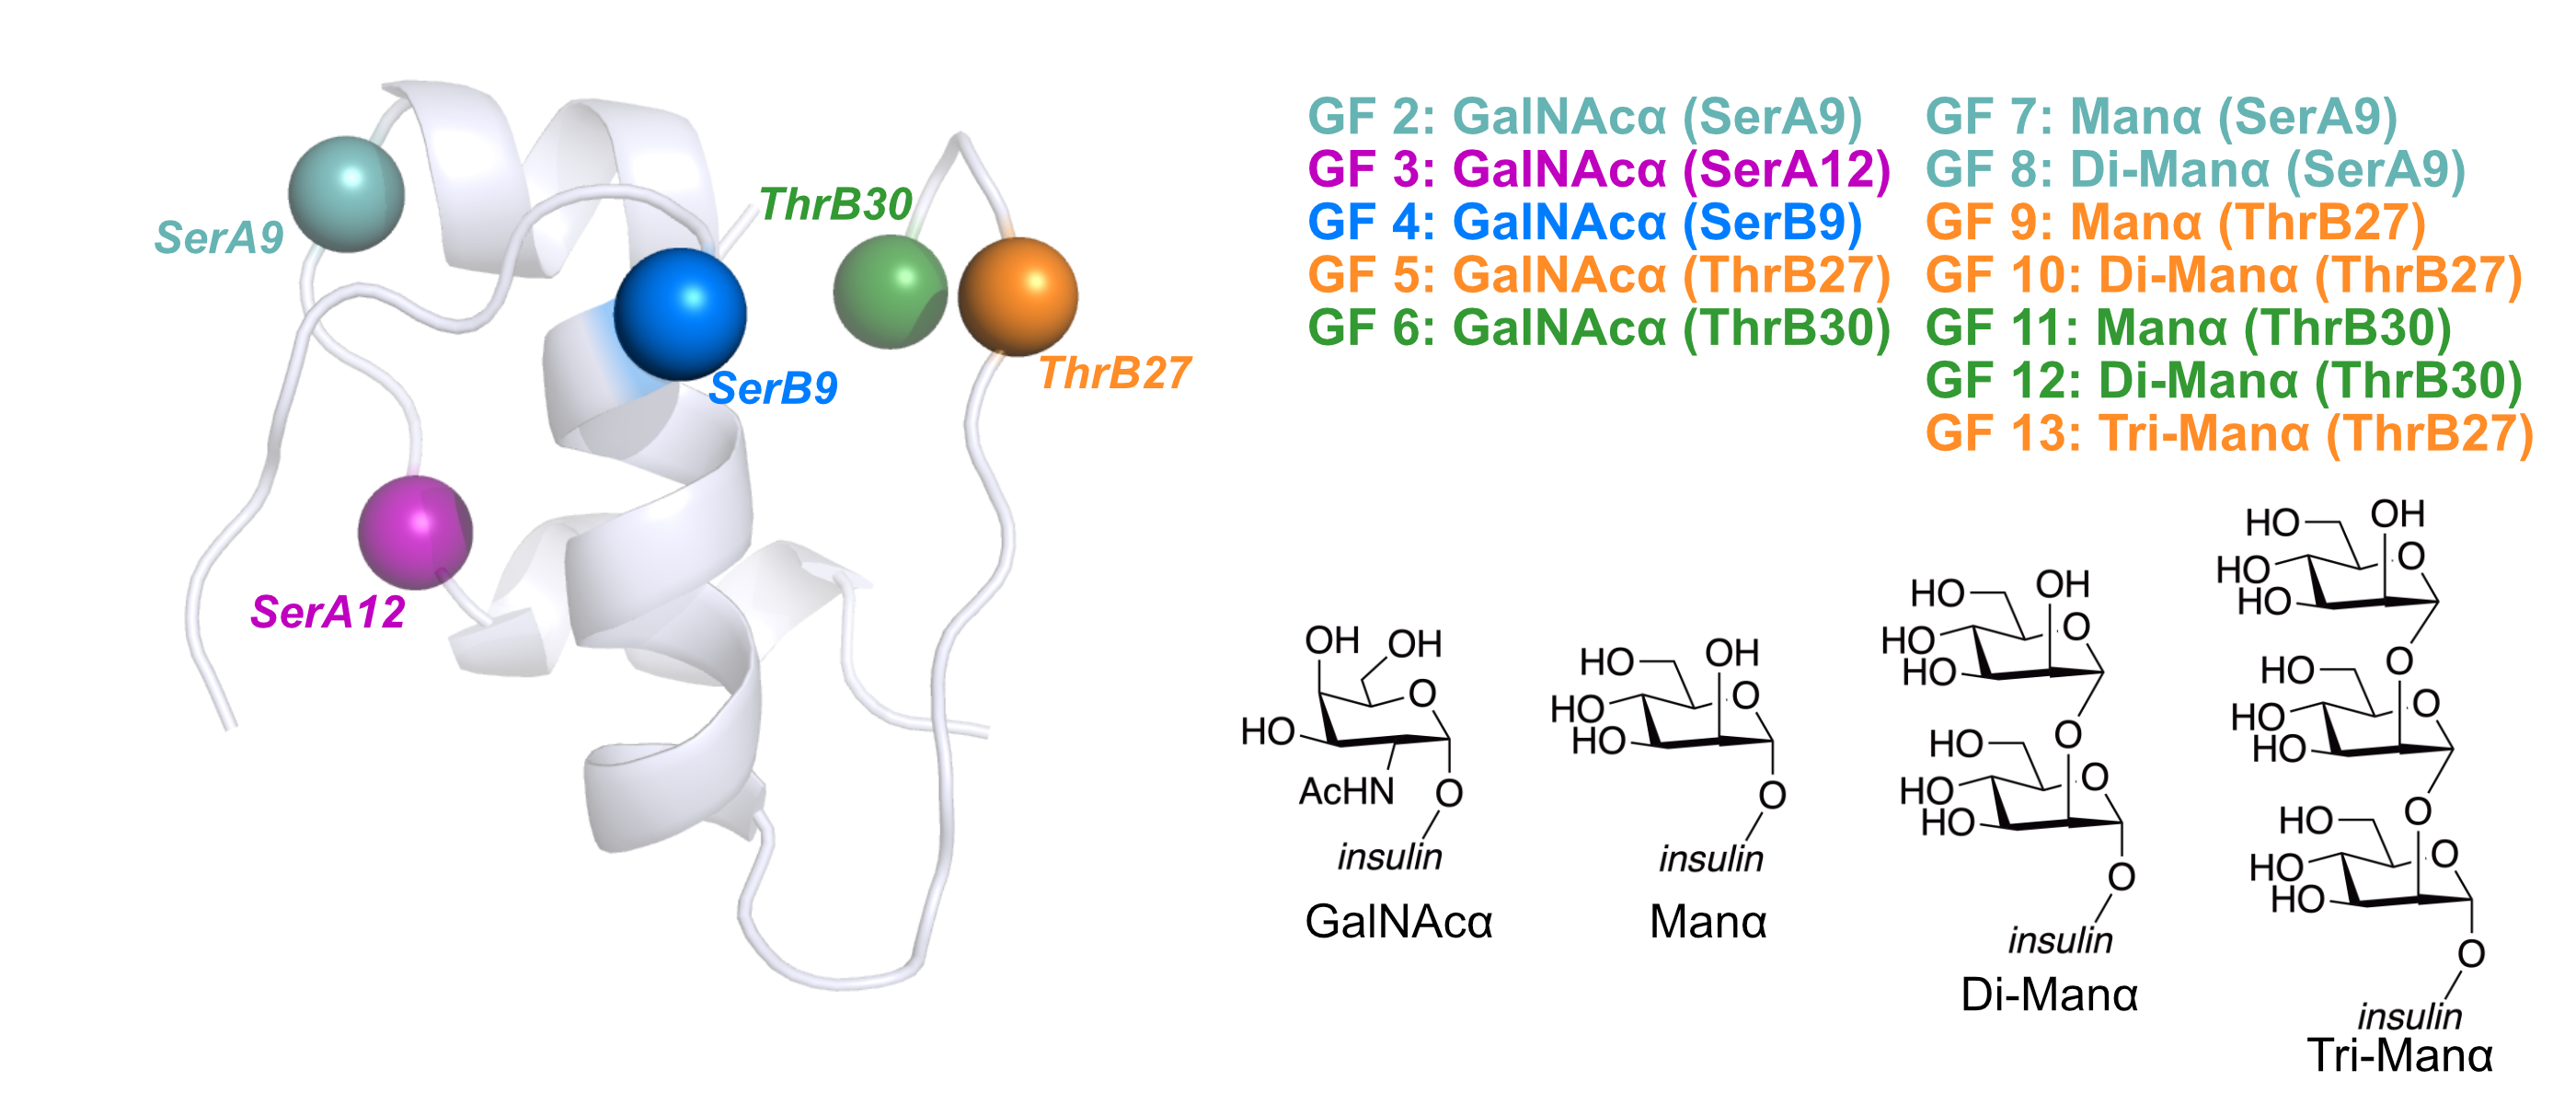
\includegraphics[width=\textwidth]{Figures/Fig_glycan_positions.png}
\caption{Structures of a human insulin monomer and glycoforms studied in this work. Two kinds of sugar moieties (\DIFdelbeginFL \DIFdelFL{N-acetylgalactosamine }\DIFdelendFL \DIFaddbeginFL \emph{\DIFaddFL{N}}\DIFaddFL{-acetylgalactosamine }\DIFaddendFL (GalNAc) and mannose (Man) in the $\alpha$-anomer) with varying lengths (e.g. a mannose monomer, dimer, or trimer) were attached to five different glycosylation sites of insulin, including SerA9 (teal), SerA12 (purple), SerB9 (blue), ThrB27 (orange) and ThrB30 (green) all represented as beads. The glycosylation pattern of each glycoform is implied by its name---for example, GalNAc$\alpha$ (SerA9) represents the glycoform having an \DIFdelbeginFL \DIFdelFL{N-acetylgalactosamine }\DIFdelendFL \DIFaddbeginFL \emph{\DIFaddFL{N}}\DIFaddFL{-acetylgalactosamine }\DIFaddendFL (GalNAc) attached to the A chain Ser9 residue. Note that for glycoforms having a mannose dimer or trimer as the glycan, the linkages between monomers were all $\alpha$-1,2-linkages, so Tri-Man$\alpha$ (ThrB27) refers to the glycoform containing an $\alpha$-1,2-linked tri-mannose at the B chain Thr27 residue.}
\label{sys_of_interest}
\end{figure}
Notably, both the proteolytic stability and dimerization propensity are related to transformation processes that require overcoming free energy barriers. The proteolytic stability can be directly associated with the free energy barrier of the formation of the conformational ensemble corresponding to the transition state in the proteolytic degradation by $\alpha$-chymotrypsin. Similarly, dimerization propensity is strongly correlated with the free energy barrier to dimerization. While these free energy differences could serve as more direct measures for the two biophysical properties of interest, calculations of such free energy differences are far from trivial. The reason lies in the fact that the timescale of the binding/unbinding events between an insulin monomer and an $\alpha$-chymotrypsin or between two insulin monomers are prohibitively long. This necessitates the use of advanced sampling techniques to accelerate the sampling of the configurational space of the system of interest, such as umbrella sampling~\cite{torrie1977nonphysical} or alchemical transformations~\cite{sugita2000replica, lyubartsev1992new}. However, such free energy methods are usually much more complicated and computationally expensive than standard MD simulations of the same length. The increase in the system size of insulin/protease complex or insulin dimer calculations adopting either method could easily increase the computational cost significantly beyond the scope of what is possible to screen large numbers of insulin modifications.  Advanced configurational sampling approaches can often be significantly difficult to set up and interpret, thus making easy screening impossible.

Therefore, instead of considering simulations of an insulin-$\alpha$-chymotrypsin complex and an insulin dimer, we worked to develop metrics for proteolytic stability and dimerization propensity based on standard MD simulations of monomers and their glycosylated analogs. The hypothesis is that the insulin monomer that participates in either a complex with $\alpha$-chymotrypsin or an insulin dimer should encode at least some important structural insights into both the proteolytic stability and the dimerization propensity. As long as we are able to explore the configurational space of monomer-based structures sufficiently, the conformational ensembles we get from the simulations should shed light on developing reasonable metrics for the two insulin properties. 

Given the output MD trajectories, all metrics were measured for each glycoform structure. They were later compared with the experimental work for assessing the efficacy. Notably, we found that at minimum 5 $\times$ 2000 ns = 10 $\mu$s of simulation was necessary to capture the structural characteristics of the insulin ensembles. This aggregate length is, to our knowledge, \DIFaddbegin \DIFadd{one of }\DIFaddend the longest among all the computational studies of human insulin. In addition, our study is not only one of the very few studies that characterize conformations of insulin with a covalently attached moiety, but is also unique as the first study that \DIFdelbegin \DIFdel{assesses }\DIFdelend \DIFaddbegin \DIFadd{correlates molecular dynamics simulations to the }\DIFaddend proteolytic stability of \DIFdelbegin \DIFdel{a protein by molecular dynamics}\DIFdelend \DIFaddbegin \DIFadd{these proteins}\DIFaddend . Our investigation facilitates a better understanding of the underlying mechanism of how different \emph{O}-glycosylation patterns influence insulin properties, which could be useful in guiding the design of insulin glyco-variants with better properties for oral delivery.
%DIF < %%%%%%%%%%%%%%%%%%%%%
%DIF < % itemized outline %%
%DIF < %%%%%%%%%%%%%%%%%%%%%
%DIF < \begin{itemize}
    %DIF <  \item Relevance: (take from existing papers and grants)
    %DIF <  \begin{itemize}
    %DIF <      \item \st{Insulin has been widely used as a peptide drug to treat diabetes by promoting the absorption of glucose from the blood. In recent years, there has been an increased interest in the development of the insulin drug for oral administration to address the low patient compliance caused by frequent subcutaneous injections(Ref 1, 2). However, the research field has been challenging due to insulin’s low permeability across the intestinal epithelium upon oligomerization and the susceptibility to proteases in the digestive system of the human body, which lead to overall low absorption efficiency. O-linked glycosylation has been considered as one of the most promising approaches to address the challenge.(Ref 3, 4). This study is aimed to apply computational methodologies to understand how specific patterns of glycosylation can help help decrease the dimerization propensity and enhance the proteolytic stability of insulin.}
    %DIF <      \item \st{We want to make insulin more stable so it’s a better treatment.}
    %DIF <      \item \st{We’d love to learn how this helps for insulin to stabilize other small protein/peptide drugs which might need even more help for stability.}
    %DIF <      \item \st{Experiments have shown that glycosylation can make insulin more proteolytically stable and less likely to dimerize (ACS 2018 paper).}
    %DIF <      \item \st{We want to investigate the ability of simulations to help screen for better glycosylation patterns, in particular identifying observables from simulations of glycosylated insulin that correlate with advantageous biophysical behavior.}
    %DIF <  \end{itemize}   
    %DIF <  \item \st{Thesis: It is important to understand, at a molecular level, the biophysical mechanisms of what glycosylation in different places can do, and computational modeling can be useful in understanding why glycosylation has the effect it does.}
    %DIF <  \begin{itemize}
        %DIF <  \item \st{Is there evidence in the literature that it useful to do simulations.}
        %DIF <  \begin{itemize}
        %DIF <      \item \st{Simulation has been used for decades to study the dynamics of insulin, including studying the dynamics of the BCCT and the energetics of dimerization/un-dimerization. These simulations have been compared to available experimental data to support their validity. See here for summaries of past literature.}
        %DIF <  \end{itemize}
        %DIF <  \item Can we capture the full unfolded nature of the terminal end of chain B.
        %DIF <  \begin{itemize}
        %DIF <      \item The B chain C terminus (BCCT) is mobile, flexible, and partially unfolded as determined by NMR. It is also known that this region must bend away from the core of the insulin molecule in order for it to bind. Several simulations have captured this mobile behavior and have generated probabilities of the BCCT separating from the core molecule. See here for summaries of past literature. It is important to capture the full flexibility of this region, especially since many of the glycoforms identified as being potentially useful are in this region or interact with it.  Looking at single crystal structures is not enough. 
        %DIF <  \end{itemize}
    %DIF <  \end{itemize}

%DIF <  \item \st{Thesis: Biophysical properties of glycosylated insulin, as elucidated by molecular dynamics, can help explain proteolytic stability and dimerization propensity.} 
    %DIF <  \begin{itemize}
    %DIF <      \item \st{Why we are focusing on these two observables.} 
    %DIF <      \item \st{What we hope might allow us to predict these biophysical observables with simulations of the monomer.} 
    %DIF <      \begin{itemize}
    %DIF <          \item \st{Why monomer instead of dimer?}
    %DIF <          \begin{itemize}
    %DIF <              \item \st{Simplify the problem of simulating two insulins by only simulating one and see if we can make predictions about dimerization without explicitly treating the dimer → quicker, more straightforward simulation procedure}
    %DIF <          \end{itemize}
    %DIF <      \end{itemize} 
    %DIF <      \item Proteolytic stability:
    %DIF <      \begin{itemize}
    %DIF <          \item \st{Association of the sugar with the most likely proteolytic cleavage site can reduce proteolysis by alpha-chymotrypsin by steric effects.}
    %DIF <          \item \st{Some hypotheses that glycosylation stiffens the cleavage site, which prevents the formation of the transition state in the cleavage reaction / Glycosylation could also reduce the propensity of formation of the transition state of the peptide in cleavage by chymotrypsin}
    %DIF <      \end{itemize}
    %DIF <      \item \st{What are the features of the ensembles of simulations of the monomer that can be used to predict dimer vs. monomer preferred states?}
    %DIF <      \item \st{Molecular simulations may help us understand how this stability occurs,}
    %DIF <  \end{itemize}
    %DIF <  \item \st{Things we are not looking at:}
    %DIF <  \begin{itemize}
    %DIF <      \item \st{Avoiding of nonspecific aggregation:}
    %DIF <      \item \st{Looking at binding to the insulin receptor as a measure of stability.}
    %DIF <  \end{itemize}
\DIFdelbegin %DIFDELCMD < 

%DIFDELCMD <     %%%
%DIF <  \item \st{Why is this study different.}
    %DIF <  \begin{itemize}
    %DIF <      \item \st{This study is unique in several ways.}
    %DIF <      \begin{itemize}
    %DIF <          \item \st{This study uses the longest simulation times (2 us x 5 structures) compared to others.}
    %DIF <          \item \st{No study has treated insulin as a conjugated protein in simulation. Few simulations have looked at the effect of non-covalent interactions between insulin and organics, but this would be first to study a covalently attached moiety.}
    %DIF <          \item \st{This would be the first study to make abstractions about dimerization using only the monomer. Others have only compared conformational dynamics between the monomer and dimer directly.}
    %DIF <          \item \st{This would be the first study to assess proteolytic stability by molecular dynamics. One previous study predicted cleavage sites by docking insulin into pepsin, but no other study has attempted to predict proteolysis by MD or with chymotrypsin.}
    %DIF <      \end{itemize}
    %DIF <  \end{itemize}
    %DIFDELCMD < 

%DIFDELCMD < %%%
%DIF < \end{itemize}
%DIFDELCMD < 

%DIFDELCMD < %%%
\DIFdelend % %===============================
% % Methodology
% %===============================
\section{Methodology}
\subsection{Molecular dynamics simulations}
\DIFdelbegin %DIFDELCMD < 

%DIFDELCMD < %%%
\DIFdelend To reduce sampling bias of our MD simulations and ensure that our analysis results were not dependent on the initial configuration of insulin, in our study, we built each of the 12 glycoforms on 5 wild-type (WT) structures resolved by different groups using different methods, whose PDB IDs were 4EYD, 4EY9, 4EY1, 3I3Z, and 2MVC, respectively (Figure \ref{starting_structures}A). These initial models were chosen based on whether they were resolved in a complex or as a monomer. For example, 4EYD, 4EY9, and 4EY1 were all crystallized in complex with Zn$^{2+}$ as a hexamer composed of a dimer in 3-fold symmetry~\cite{favero2013structural}. They represented high-resolution human insulin structures from pharmaceutical formulations. 3I3Z and 2MVC, on the other hand, were representative of monomeric insulin structures. 3I3Z was resolved by X-ray crystallography under low gravity conditions so that the asymmetric unit of insulin was a monomer~\cite{timofeev2010x}. 2MVC was resolved by NMR spectroscopy under acidic conditions, which \DIFdelbegin \DIFdel{were }\DIFdelend \DIFaddbegin \DIFadd{is }\DIFaddend known to favor the monomeric form of insulin~\cite{kvrivzkova2014structural}.

For those models resolved in the dimeric form, including 4EYD, 4EY9, and 4EY1, we extracted the insulin monomer from the dimer conformation. For 3I3Z, which was resolved as a monomer with the last residue on the B-chain mutated into an alanine, we used PyMOL~\cite{delano2002pymol} to mutate the residue back to a threonine to match the standard sequence of human insulin. Lastly, for the NMR-resolved 2MVC, we simply took the first model from the PDB file of the resolved ensemble. Notably, even if monomers extracted from a dimer conformation could potentially suffer from biases from experimental conditions that favor dimer resolution, as later shown, these biases did not have noticeable influences on the consistency of our methods. 

\begin{figure}[H]
\centering
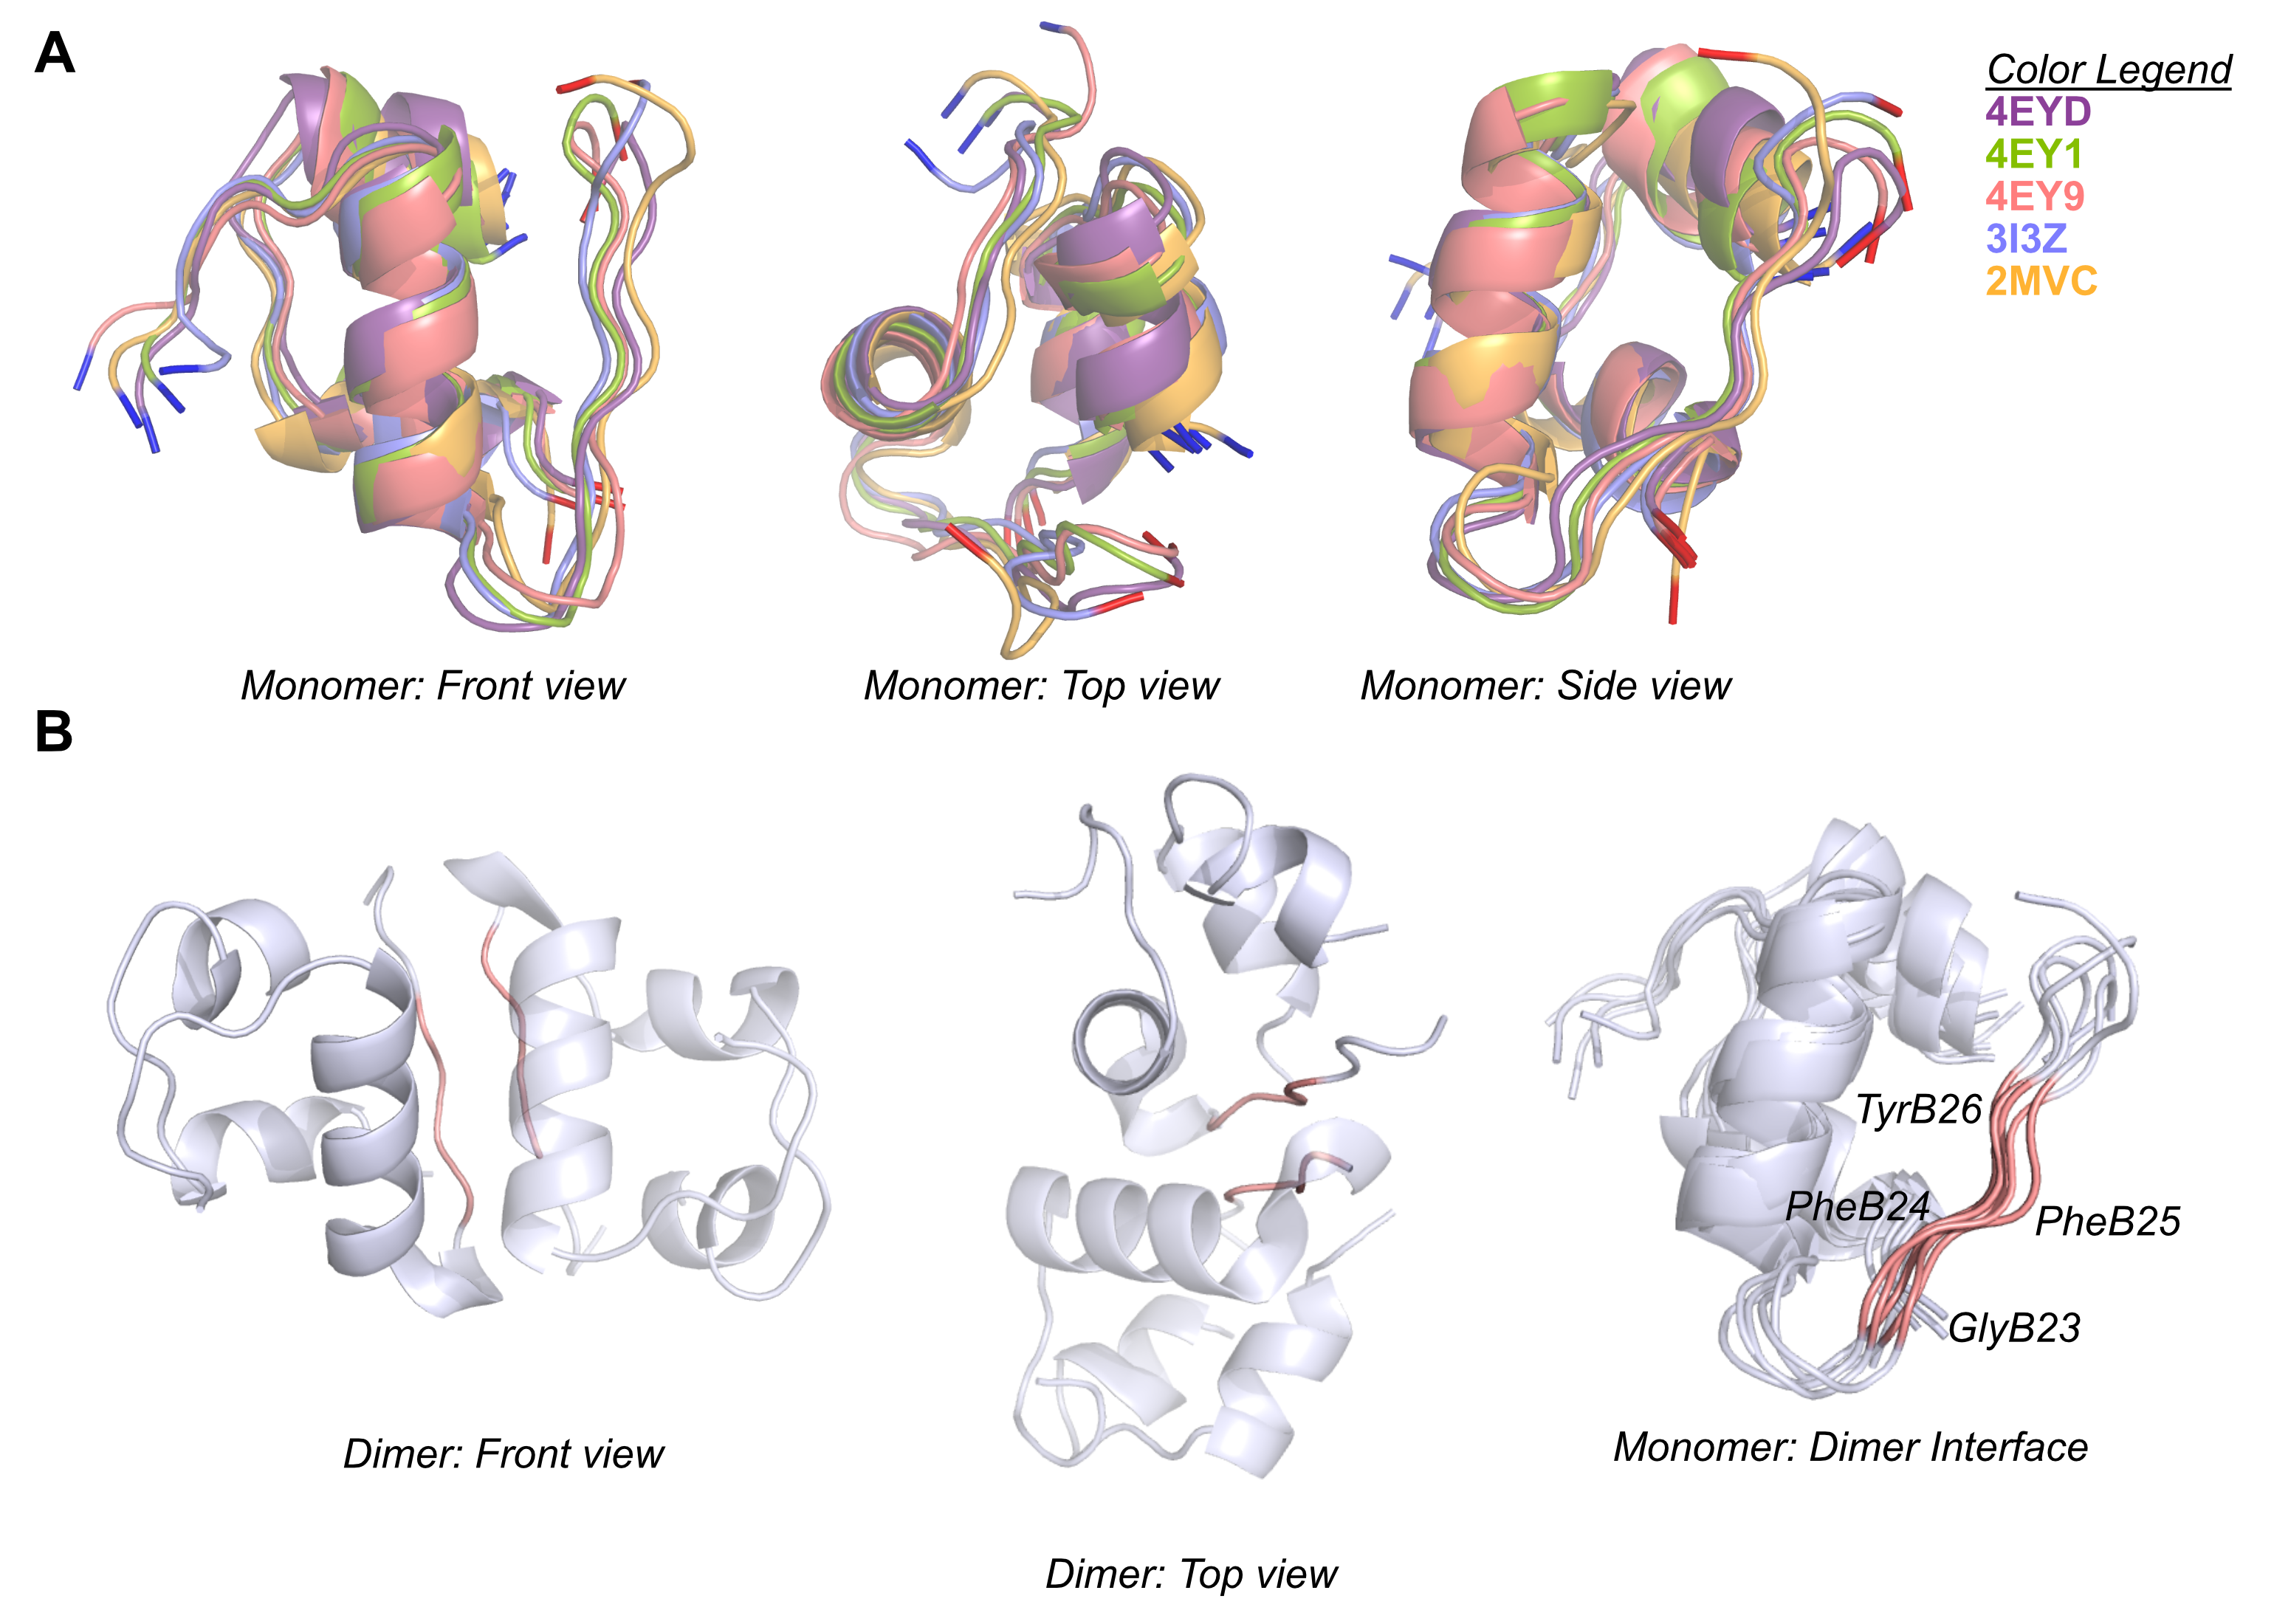
\includegraphics[width=\textwidth]{Figures/Fig_WTmodels_dimerInterface.png}
\caption{Structures of wild-type insulin models used in this study. (A) The initial monomer structures, after equilibration and before production simulation, are superimposed and are shown from different views. (B) Representative dimer structure illustrating the dimerization interface. The 3I3Z crystal structure was used to reconstruct an insulin dimer in the first two images. Residues GlyB23--TyrB26 (salmon) are highlighted. The last image shows the superimposed equilibrated wild-type structures with \DIFaddbeginFL \DIFaddFL{residue }\DIFaddendFL labels for the dimer interface.}
\label{starting_structures}
\end{figure}

After extracting the monomer structure from each of the initial models, we used the H++ server (version 3.2)~\cite{anandakrishnan2012h++, myers2006simple, gordon2005h++}\DIFaddbegin \DIFadd{, which also parameterized the protein with the AMBER ff14SB force field, }\DIFaddend to assign reasonable protonation states \DIFdelbegin \DIFdel{under the pH value (8.0) }\DIFdelend \DIFaddbegin \DIFadd{corresponding to the pH values }\DIFaddend adopted in experiments. \DIFdelbegin \DIFdel{At }\DIFdelend \DIFaddbegin \DIFadd{Specifically, in the work~\mbox{%DIFAUXCMD
\cite{guan2018chemically} }\hspace{0pt}%DIFAUXCMD
by Guan et al., the experiments of $\alpha$-chymotrypsin digestion (for estimating the $\alpha$-chymotrypsin half-life, hence the proteolytic stability) and analytical ultracentrifugation (for estimating the monomer/dimer population, hence the dimerization propensity) were conducted at }\DIFaddend pH 8.0 \DIFdelbegin \DIFdel{, the }\DIFdelend \DIFaddbegin \DIFadd{and pH 7.4, respectively. These two pH values respectively correspond to the typical pH values in the pancreatic tract (pH 7.5 to pH 8.0 ~\mbox{%DIFAUXCMD
\cite{mcqueen2017comprehensive}}\hspace{0pt}%DIFAUXCMD
) and small intestine (pH 6 to pH 7.4~\mbox{%DIFAUXCMD
\cite{fallingborg1999intraluminal}}\hspace{0pt}%DIFAUXCMD
) of human body. Around these pH values, the }\DIFaddend total charges of insulin were predicted to be -1 or -2,  depending on the pK$_{1/2}$ value of the two histidine residues (HisB5 and HisB10) of insulin. We \DIFdelbegin \DIFdel{therefore }\DIFdelend \DIFaddbegin \DIFadd{then }\DIFaddend adjusted the external pH value in H++ of each wild-type structure to \DIFdelbegin \DIFdel{make sure all of them had }\DIFdelend \DIFaddbegin \DIFadd{give }\DIFaddend total charges of \DIFdelbegin \DIFdel{-2. }\DIFdelend \DIFaddbegin \DIFadd{-1. Notably, this value of total charge was preferred to -2 because it collectively corresponded to pH values ranging from 6.6 to 7.8 (see Supplemental Table S3), which overlapped both the pH ranges in the small intestine and the pancreatic tract. If a total charge of -2 were adopted, the corresponding pH ranges would have been higher and not able to overlap the typical pH range of the small intestine.
}

\DIFaddend Simulated structures from 4EYD, 4EY1, and 3I3Z had exactly the same protonation state for each residue. 4EY9 and 2MVC, on the other hand, were found to have \DIFdelbegin \DIFdel{protonation states for the histidine residues different from }\DIFdelend \DIFaddbegin \DIFadd{different histidines protonated compared to }\DIFaddend the ones in the other three models (see Supplemental Table \DIFdelbegin \DIFdel{S1}\DIFdelend \DIFaddbegin \DIFadd{S3}\DIFaddend ).  We chose to include this ensemble of protonation sites, as they were essentially attributable to the orientations of the histidine residues and their surroundings. In addition, these two histidine residues were far away from the residues involved in the hypotheses of our analysis methods (see Supplemental Figure \DIFdelbegin \DIFdel{S1}\DIFdelend \DIFaddbegin \DIFadd{S6}\DIFaddend ), making them less likely to have noticeable influences on the predictors we developed. We started from these parameterized wild-type insulin conformations with reasonable protonation states and used GLYCAM glycoprotein builder~\cite{kirschner2008glycam06}, which \DIFdelbegin \DIFdel{utilized }\DIFdelend \DIFaddbegin \DIFadd{used the }\DIFaddend GLYCAM06j-1 force field, to build various glycoform structures by attaching different saccharide moieties to the corresponding glycosylation sites. 

In this study, the simulations of all wild-type and glycoform structures were performed using GROMACS 2020.4~\cite{abraham2015gromacs, pall2014tackling} at 310.15 K, which was in agreement with experimental temperature. Outputs in AMBER formats generated by GLYCAM glycoprotein builder were converted into GROMACS formats using ACPYPE~\cite{da2012acpype} to serve as the inputs of the simulations. Each structure was solvated in a dodecahedral box with 1.0 nm between the solute and the box edge. Sodium and chloride ions were added to neutralize the system and match the specified salinity of 0.15 M. The system was then energy minimized with the steepest descent algorithm until the maximum force was lower than 100.0 kJ/mol/nm. Subsequently, a 200 ps NVT equilibration followed by a 200 ps NPT equilibration was carried out, in which the Berendsen barostat~\cite{berendsen1984molecular} and velocity rescaling~\cite{bussi2007canonical} were employed to maintain the reference temperature and pressure at 310.15K and 1 bar, respectively. Finally, an MD simulation was performed in an NPT ensemble, with the pressure maintained at 1 bar by the Parinello-Rahman barostat~\cite{parrinello1980crystal, parrinello1981polymorphic}. The cut-off distances for van der Waals interactions and Coulomb interactions were both set as 0.9 nm, with \DIFdelbegin \DIFdel{swiching }\DIFdelend \DIFaddbegin \DIFadd{the switching }\DIFaddend of the van der Waals potential between 0.85 and 0.9 nm and an analytical correction for \DIFdelbegin \DIFdel{long range }\DIFdelend \DIFaddbegin \DIFadd{long-range }\DIFaddend dispersion. The particle mesh Ewald algorithm~\cite{essmann1995smooth} was used with real-space switching of the potential between 0.89 nm and 0.9 nm. LINCS~\cite{lincs} was used to constrain hydrogen bonds. All the simulations were extended up to 2000 ns, which we deemed necessary to capture insulin dynamics in which the major transitions between metastable states occurred on the time scale of \DIFdelbegin \DIFdel{500--2000ns}\DIFdelend \DIFaddbegin \DIFadd{500--2000 ns}\DIFaddend , as interpreted from \DIFaddbegin \DIFadd{the }\DIFaddend time series of the pairwise RMSD calculations of the wild-type structures (see Supplemental Figure \DIFdelbegin \DIFdel{S2).  }\DIFdelend \DIFaddbegin \DIFadd{S1).  Our simulations captured the key important disordered elements investigated by Busto-Moner et al.~\mbox{%DIFAUXCMD
\cite{busto2021structural}}\hspace{0pt}%DIFAUXCMD
,  though at different percentages. This discrepancy is not surprising given the pH difference between the two studies, with the differences elaborated in Section 1 in the supporting information.  }\DIFaddend All trajectories were stored every 250 ps, for a total of 8001 frames for analysis. All the input configurations and GROMACS mdp files are provided in the \DIFdelbegin \DIFdel{GitHub repository}\DIFdelend \href{https://github.com/shirtsgroup/Glycoinsulin_project}{\DIFdelbegin \DIFdel{https://github.com/shirtsgroup/Glycoinsulin\_project}\DIFdelend \DIFaddbegin \DIFadd{GitHub repository}\DIFaddend } for this study.

%DIF < %%%%%%%%%%%%%%%%%%%%%
%DIF < % itemized outline %%
%DIF < %%%%%%%%%%%%%%%%%%%%%
%DIF <  \begin{itemize}
    %DIF <  \item \st{Five wild type structures were adopted to serve as the basis to build glycoform structures, including 4EYD, 4EY9, 4EY1, 3I3Z and 2MVC.}
    %DIF <  \begin{itemize}
    %DIF <      \item \st{Why we chose these.}
    %DIF <      \begin{itemize}
    %DIF <          \item \st{Initial models were chosen based on whether they were solved in a complex or as a monomer, and multiple models were chosen to reduce sampling bias. Three of these (4EYD, 4EY9, and 4EY1) represent high-resolution structures from pharmaceutical preparations. They all represent normal human insulin and were crystallized with Zn in complex therefore might be pre-biased for dimer conformation.}
    %DIF <          \item \st{More details about 3I3Z and 2MVC. We might want to make sure if 2MVC is biased or not. (Some of its results deviate from results obtained from glycoforms based on other wild type structures.)}
    %DIF <          \item \st{3i3z - solved under low gravity conditions so that the asymmetric unit was a monomer i.e. representative monomeric insulin structure. Structure might be pre-biased for the monomer (ref)}
    %DIF <          \item \st{2mvc - solved under acidic conditions by NMR, acid is known to keep the structure in monomeric form. Structure might be pre-biased for monomer conformation (ref)}
    %DIF <          \item \st{Including structures with dimer and monomer biases should clarify the role this plays in interpreting results}
    %DIF <      \end{itemize}   
    %DIF <  \end{itemize}
    \DIFdelbegin %DIFDELCMD < 

%DIFDELCMD <     %%%
%DIF <  \item \st{How were glycoforms selected?}
    %DIF <  \begin{itemize}
    %DIF <      \item \st{Glycoforms studied in 2018 ACS Chem Bio paper, We have proteolytic data and dimerization data in some instances.}
    %DIF <      \item \st{Fig. chemical structure of glycoforms. (incorporate the chemical structure differences) }
    %DIF <      \item \st{MR: Fig. 3D strucuture of one of the isoforms OR, superposition of all isoforms on the same pdb structure (different color). OR all 5 next to each other: protein in translucent gray for all of them and the sugar in color.}
%DIFDELCMD < 

%DIFDELCMD <     %%%
%DIF <  \end{itemize}
    %DIFDELCMD < 

%DIFDELCMD <     %%%
%DIF <  \item \st{How do we choose wild type insulin initial structure for the control, and for glycosylating?}
    %DIF <  \begin{itemize}
    %DIF <      \item \st{Sets of glycoforms were built from all of the 5 insulin models. Each WT model serves as the control for the set of glycoforms built from it.}
    %DIF <  \end{itemize}
    %DIFDELCMD < 

%DIFDELCMD <     %%%
%DIF <  \item \st{For each wild type structure, we build 12 glycoforms described in the 2018 ACS paper.}
    %DIF <  \item \st{For each glycoform, we performed a standard MD simulation for 2000 ns at 310.15 K and a neutral pH value, which are consistent with the experimental conditions of the cleavage reaction conducted in ACS 2018 paper. We made sure that the protonation states of different wild type structures are as consistent as possible.}
    %DIF <  \begin{itemize}
    %DIF <      \item \st{How do we decide if the simulation is long enough? → There is no apparent transition in the RMSD values (need to check for all the glycoforms).}
    %DIF <      \begin{itemize}
    %DIF <          \item \st{We ran 500 ns, but it looked like the RMSD’s were statistically different between different structures of wild type insulin, so we ran 2000 ns and they became statistically similary, so we stopped making the, longer.}
    %DIF <          \item \st{DSSP Helix assignment autocorrelation times were on the order of 30-1000ns, so 2000ns was judged to be minimally acceptable to ensure we captured this event.}
    %DIF <          \item \st{Description of supplemental table: list of helix structure autocorrelation times} 
    %DIF <      \end{itemize}   
    %DIF <      \item \st{Add a figure of RMSD as a function of time in the SI showing that 2000 ns is enough.} 
    %DIF <      \begin{itemize}
    %DIF <          \item \st{There are 65 glycoforms, how do we pick which to plot?}
    %DIF <      \end{itemize}
    %DIF <      \item \st{!0 us total per glycoform, if we can’t successfully with this amount of simulation, other avenues should be explored.} 
    %DIF <  \end{itemize}
    %DIFDELCMD < 

%DIFDELCMD <     
%DIFDELCMD <     %%%
%DIF <  \item \st{Justification of difference in protonation states (might be too detailed even in the paper?)}
    %DIF <  \begin{itemize}
    %DIF <      \item \st{As mentioned in the 2018 ACS paper, the measurements of the chymotrypsin half-life for each insulin glycoform was taken at pH 8.0. To predict the protonation states of each wild type structure at this pH value and make them as consistent, we first used H++ to predict the total charges of each wild type setting the pH value as 8. The resulting total charges of structure could be either -1 or -2, majorly depending on the protonation state of HisB5, whose midpoint of the titration curve (pK\_{1/2}) is generally very close to 8.0.}
    %DIF <      \item \st{To make the protonation states of different wild type structures as consistent as possible, we first tweaked the pH value for H++ parameterization such that all the wild type structures had total charges as -1. (The resulting pH values for 4EYD, 4EY9, 4EY1, 3I3Z and 2MVC were 8.0, 8.0, 7.9, 6.9, and 7.3, respectively.) Then, we compared the protonation state of different wild type structure residue by residue. As a result, wild type structures 4EYD, 4EY1, and 3I3Z had exactly the same protonation state for each residue. On the other hand, despite having total charges of -1,  2MVC and 4EY9 were found to have different protonation states at some of the histidine residues, whose pK value could be fluctuating around 8.0 depending on its configuration and the surroundings (Ref). }
    %DIF <      \item \st{Specifically, the protonation state of HisB10 in 4EY9 was predicted to be HID, which was different from that of 4EYD, 4EY1 and 3I3Z (HIE). As both HID and HIE states are uncharged, this did not lead to a difference in the total charges. }
    %DIF <      \item \st{The protonation states of HisB5 and HisB10 of 2MVC are HIE (+0) and HIP (+1), respectively, which is the reverse of the two residues of 4EYD, 4EY1 and 3I3Z and also does not result in a difference in the total charges.}
    %DIF <      \item \st{Below is a table summarize the protonation states of histidine residues for each wild type:}
    %DIF <      \begin{center}
    %DIF <      \begin{tabular}{|c|c|c|c|c|c|}
        %DIFDELCMD < 

%DIFDELCMD <     %%%
%DIF <      \hline
    %DIF <           & 4EYD & 4EY1 & 3I3Z & 4EY9 & 2MVC \\
    %DIF <      \hline
    %DIF <      HisB5 & HIP (+1) &HIP (+1) &HIP (+1) &HIP (+1) & HIE (+0) \\
    %DIF <      \hline
    %DIF <      HisB10 & HIE (+0) & HIE (+0) &HIE (+0) &HID (+0) & HIP (+1)  \\
    %DIF <      \hline
    %DIF <      \end{tabular}
    %DIF <      \end{center}
%DIF <          \item \st{Upon molecular visualization, it was found that both histidine residues were far from the tail region of chain B in insulin, which was the key region for proteolytic degradation (Ref), so we concluded that this difference should not influence our study in dimerization propensity and proteolytic stability. (Add a figue in SI.)}
%DIF <          \item \st{For dimerization assessment, only residues B17-26 were considered because this region contains the known interfacial residues (ref 1, ref 2, ref 3) that are key for forming the dimer. The central helix in chain B is important for making intramolecular interactions with this dimer interface, but only the dimer interface is important for the dimerization event.}
%DIF <          \item \st{It’s difficult to tell what the RIGHT isoelectric protonation state is, because different structures get different protonation states, so we can’t say a priori which is right, and it’s likely it exists in an equilibrium in solution.}  
%DIF <          \item \st{We do some basic checks to make sure that the results are not statistically different between the differently protonated states. In particular, 2MVC where the protonation is on different residues. 4EY9 as well. ONE PARAGRAPH IN RESULTS ON THIS.}
%DIF <      \end{itemize}
%DIF <      \item \st{The glycosylated moieties  were built using GLYCAM, which utilized AMBER ff12SB force field. On the other hand, the wild type insulin was parameterized using H++, which used AMBER ff14SB force field.}
%DIF <      \item \st{How dependent are the results on the choice of initial insulin structure?}
%DIF <  \end{itemize}
%DIFDELCMD < 

%DIFDELCMD < %%%
\DIFdelend \subsection{Analysis techniques} \label{analysis_method}
\subsubsection{Proteolytic degradation}
\paragraph{Metric 1: SASA of the scissile bonds}
$\alpha$-chymotrypsin is a common digestive protease secreted by the pancreas which performs proteolysis in the duodenum~\cite{wilcox19705}. Experimental work~\cite{guan2018chemically} used $\alpha$-chymotrypsin to assess the proteolytic stability by measuring the half-life of different insulin glycoforms. In proteolytic degradation of insulin by $\alpha$-chymotrypsin, residues including TyrA14, TyrA19, TyrB16, PheB25, and TyrB26 serve as the cleavage sites, whose scissile bonds are on the carboxyl side~\cite{schilling1991degradation}. Previous research into $\alpha$-chymotrypsin~\cite{schilling1991degradation} indicated that residues PheB25 and TyrB26 were the cleavage sites considered to be the most susceptible to proteolytic stability. We therefore hypothesized that the exposure of the scissile bonds of these two residues to the solvent was positively correlated with proteolytic susceptibility. 

To quantify the solvent exposure of these sites, we used the double cubic lattice method (DCLM)~\cite{eisenhaber1995double} to calculate the SASA of the CONH atoms, which were the atoms sharing the same plane with the scissile bond, between PheB25 and TyrB26, and between TyrB26 and ThrB27. In DCLM, the accessible surface is defined by tracing the center of the probe sphere (with the radius as the van der Waals radius of water) as it rolls along the van der Waals surface of the solute.  The obtained SASA time series was truncated to discard the non-equilibrium region and was then decorrelated~\cite{chodera2016simple}. The mean and the standard deviation of the time series were calculated for each glycoform. Finally, the reported value for each glycoform is the value averaged across the five different wild-type bases, with the uncertainty being the standard deviation of the 5 runs. We then plotted the $\alpha$-chymotrypsin half-life measured in the experimental work against these averaged SASA values in a correlation plot, with the Kendall's tau correlation coefficient ($\tau$)~\cite{kendall1948advanced} and its \DIFdelbegin \DIFdel{corresponding two-tailed p-value determined. }\DIFdelend \DIFaddbegin \DIFadd{uncertainty annotated. The uncertainty of the correlation coefficient was estimated from bootstrapping, as detailed in section \ref{bootstrap}. Note that }\DIFaddend Kendall's tau was \DIFdelbegin \DIFdel{used as }\DIFdelend \DIFaddbegin \DIFadd{adopted in favor of Pearson correlation coefficient because }\DIFaddend it was not clear \DIFdelbegin \DIFdel{that the relationship }\DIFdelend \DIFaddbegin \DIFadd{if the relationship between the two variables }\DIFaddend should be linear, so we \DIFdelbegin \DIFdel{are assuming }\DIFdelend \DIFaddbegin \DIFadd{assume }\DIFaddend only a monotonic relationship.

\paragraph{Metric 2: SASA of the P1 sites}
In addition to the cleavage sites PheB25 and TyrB26, we hypothesized that their adjacent residues along the \emph{N}-terminal direction, namely, the P1 residues according to Schechter-Berger nomenclature~\cite{schechter1968active} were also important. \DIFaddbegin \DIFadd{In Schechter-Berger nomenclature, the residues N-terminal to the cleavage site are denoted as P1, P2, P3, \ldots etc., while the residues in the opposite direction are denoted as P1', P2', P3' ... etc. See Figure \ref{P_sites}. }\DIFaddend Specifically, the hydrophobicity of the P1 residue was found to be important in the molecular recognition of $\alpha$-chymotrypsin~\cite{appel1986chymotrypsin}, as the deep hydrophobic pocket formed by Ser189, Gly216, and Gly226 in $\alpha$-chymotrypsin requires the P1 residue to be hydrophobic as well~\cite{hedstrom2002serine}. Given the fact that the P1 residue itself needed to be sufficiently solvent-exposed to contact and fit in this hydrophobic pocket of $\alpha$-chymotrypsin, we hypothesized that a glycoform would be more proteolytically stable if its P1 sites were less solvent accessible due to the steric hindrance by the glycan moiety. Therefore, we calculated the residue SASA of PheB24 and PheB25, which were the P1 sites corresponding to the cleavage sites PheB25 and TyrB26, respectively. DCLM was used to generate the SASA time series, which was then truncated and decorrelated with the same method as the one used in Metric 1. Similarly, the final reported value of each glycoform is the value averaged across simulations starting from the five different wild-type structures, with the uncertainty being the standard deviation of the 5 runs. The monotonicity of the relationship between the metric and the experimental data was assessed by \DIFdelbegin \DIFdel{the }\DIFdelend Kendall's tau correlation coefficient ($\tau$)~\cite{kendall1948advanced}, with \DIFdelbegin \DIFdel{the corresponding two-tailed p-value calculated }\DIFdelend \DIFaddbegin \DIFadd{its uncertainty calculated using the method described in section \ref{bootstrap}. Additionally, in the supporting information (Figures S4), we examined the correlations between any two of the four SASA measures in Metric 1 and Metric 2, including the scissile bond SASA of B26--B27 and P1 site SASA of residues B24 and B25}\DIFaddend . 

\paragraph{Metric 3: $\beta$-sheet propensity of the P1--P3 region}
Previous experimental studies~\cite{bode1993natural,hedstrom2002serine,coombs1999revisiting} of $\alpha$-chymotrypsin complexes revealed an invariant feature that the polypeptide binding sites of $\alpha$-chymotrypsin formed a short antiparallel $\beta$-sheet with the backbone atoms of the P1--P3 sites of the substrate. In the case of insulin as the substrate, considering the P1 to P3 sites of both important cleavage sites (PheB25 and TyrB26) leads to residues including ArgB22, GlyB23, PheB24, and PheB25. As such, we hypothesized that glycoforms whose ArgB22 to PheB25 residues had lower $\beta$-sheet propensity would destabilize the transition state in the protease-substrate binding event, hence decreasing the proteolytic susceptibility. This assumption also stemmed from the fact that drastic structural re-orientations or even secondary structure transformations of the insulin substrate cost free energy and disfavored proteolysis accordingly. To evaluate the $\beta$-sheet propensity of these sites, we calculated the $\psi$ and $\phi$ angles of the residues. We then used MDAnalysis~\cite{gowers2019mdanalysis, michaud2011mdanalysis} to locate all the frames in a Ramachandran plot~\cite{ramachandran1963stereochemistry} and defined the $\beta$-sheet propensity as the fraction of the points in the $\beta$-sheet region defined by Lovell et al.~\cite{lovell2003structure} Again, for each glycoform, we report the fractions averaged across different wild-type bases, with the uncertainty \DIFaddbegin \DIFadd{reported as }\DIFaddend the standard deviation \DIFdelbegin \DIFdel{over runs }\DIFdelend \DIFaddbegin \DIFadd{of the mean over simulations }\DIFaddend with the five different initial structures. Finally, the $\alpha$-chymotrypsin half-life was plotted against these averaged $\beta$-sheet fractions in a correlation plot, where the Kendall's tau correlation coefficient ($\tau$) and its \DIFdelbegin \DIFdel{corresponding two-tailed p-value were determined }\DIFdelend \DIFaddbegin \DIFadd{uncertainty were determined using the bootstrap method described in section \ref{bootstrap}}\DIFaddend . The Ramachandran plot of each of the 4 residues of interest of each glycoform can be found in our \href{https://github.com/shirtsgroup/Glycoinsulin_project}{GitHub repository}. \DIFaddbegin \DIFadd{Additionally, in the supporting information (Figures S5 and S6), we examined the correlations between any two of the four measures (B22-B25) of the $\beta$-sheet propensity metric and the correlations between any SASA measure in Metric 1 or Metric 2 and any $\beta$-sheet propensity measure in Metric 3. 
}\DIFaddend 

\DIFaddbegin \begin{figure}[H]
\centering
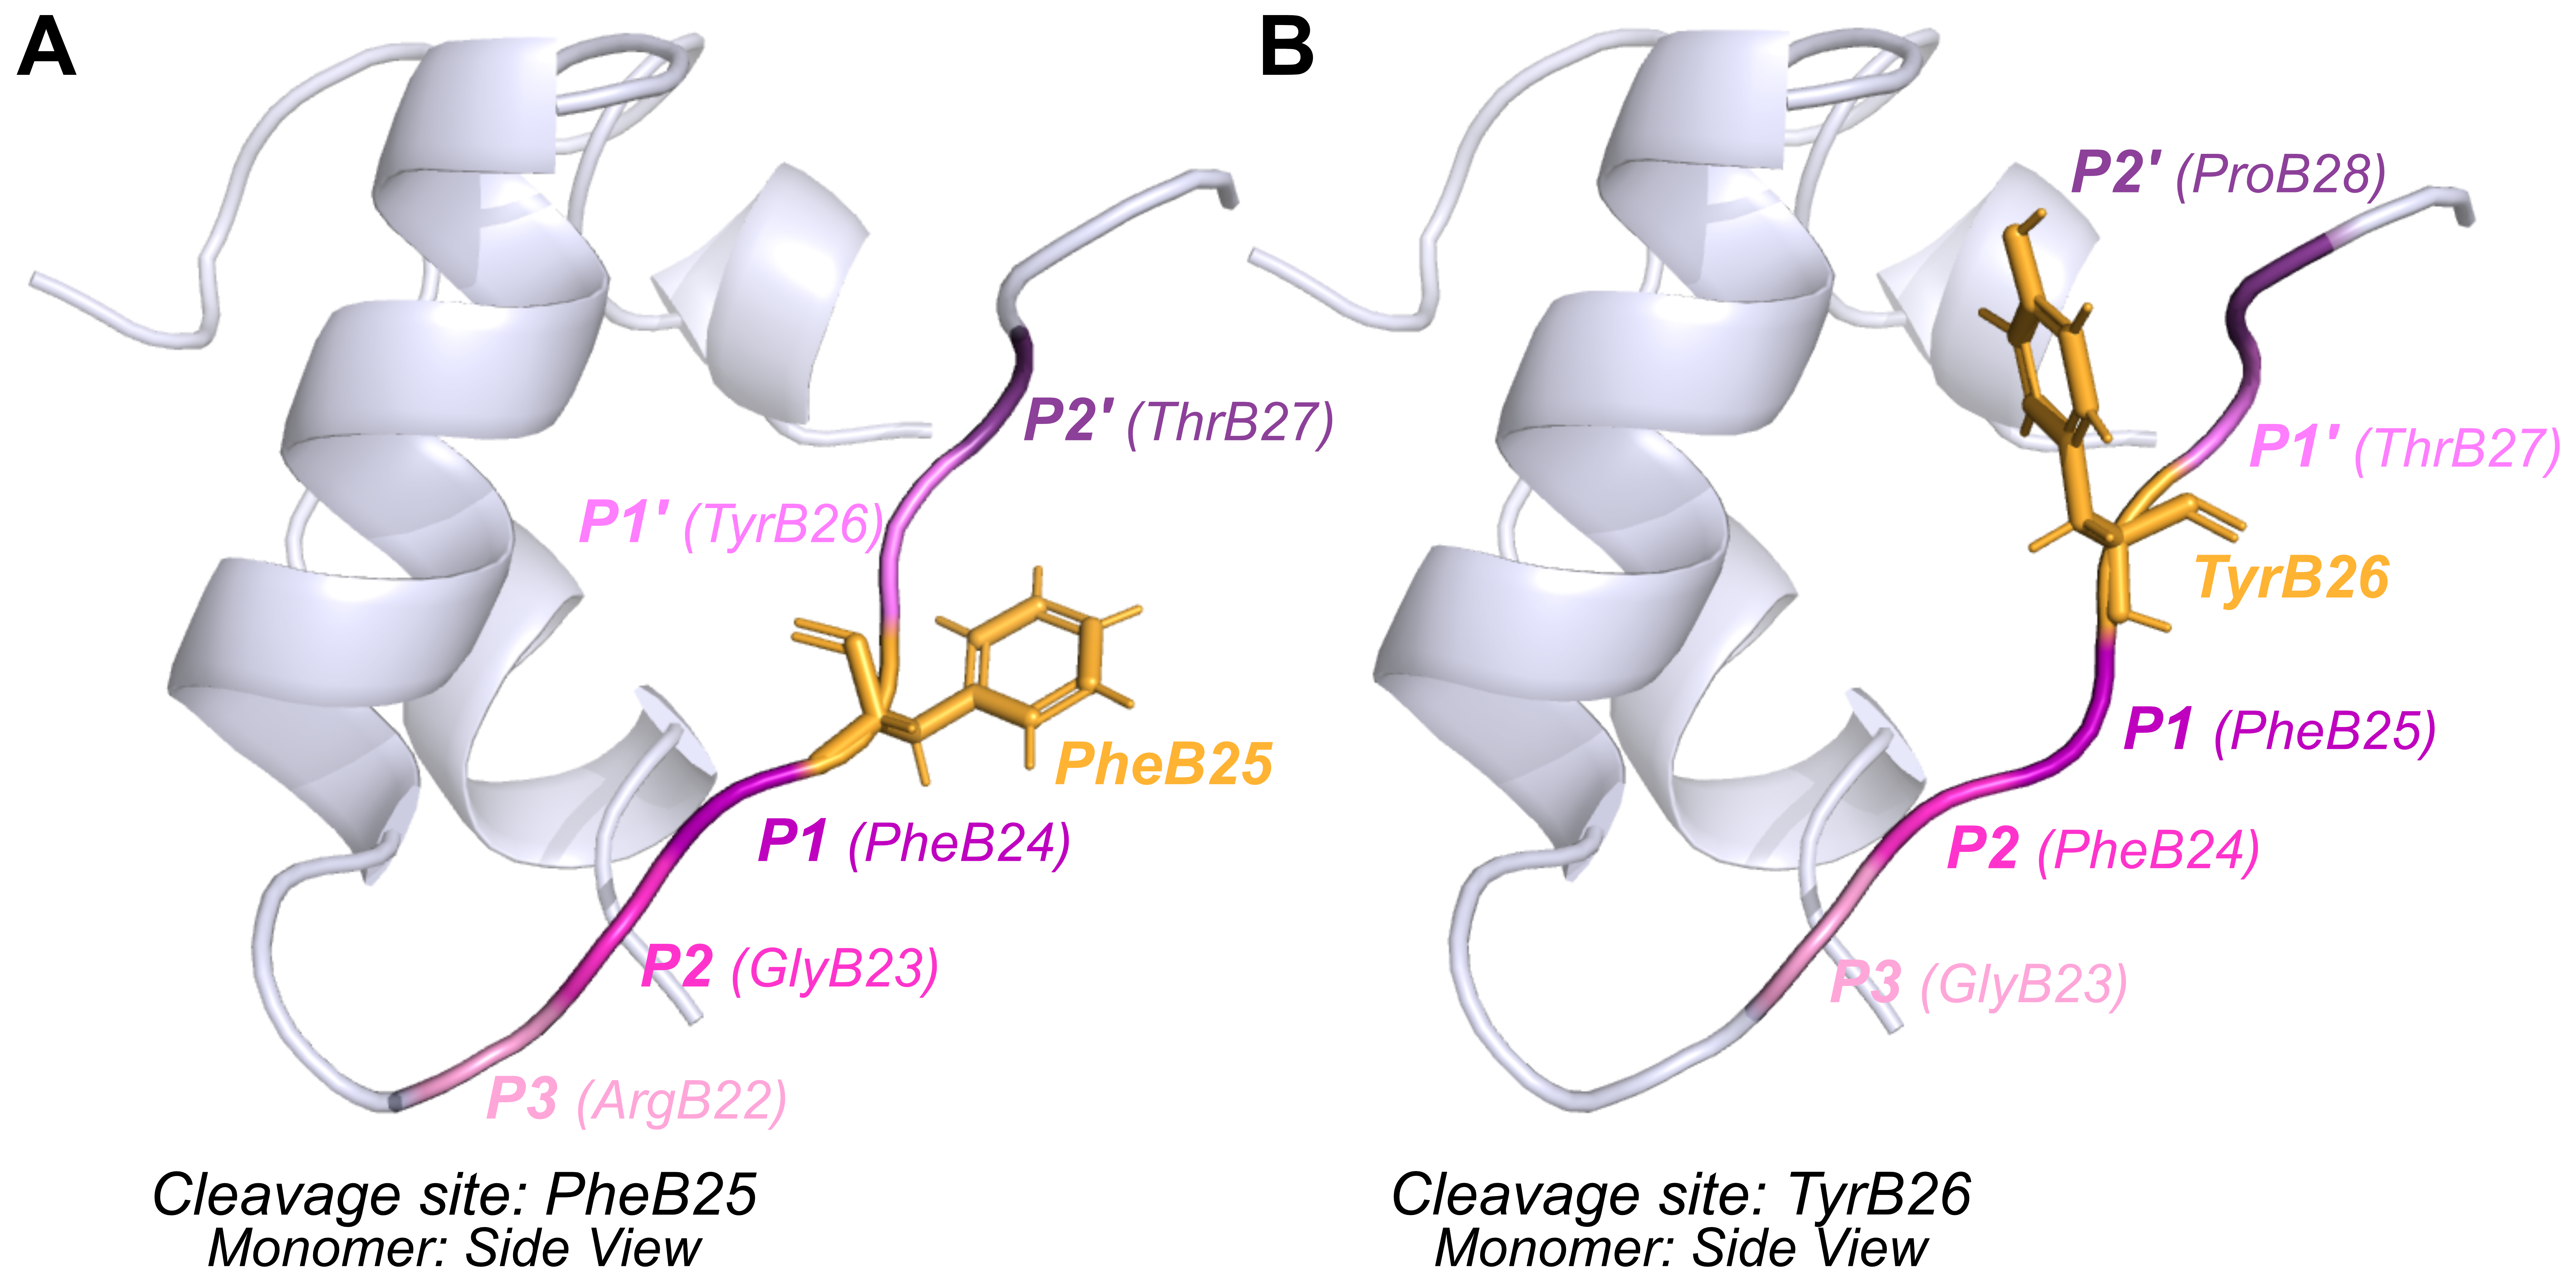
\includegraphics[width=0.95\textwidth]{Figures/P_sites.png}
\caption{\DIFaddFL{The P- and P'-sites of the two most important cleavage sites, residues PheB25 and TyrB26. The cleavage sites are shown as  orange sticks, while the remaining part of the protein is shown in cartoon representation. Schechter-Berger nomenclature for residues surrounding the cleavage sites are shown in varying shades of magenta and are labeled P1-3 and P1'-2'.}}
\label{P_sites}
\end{figure}

\DIFaddend \paragraph{Metric 4: Existence of glycan-involved hydrogen bonds}
In addition to the consensus conformations of the binding sites, some of the hydrogen bonds between $\alpha$-chymotrypsin and the substrate were also found crucial for efficient substrate hydrolysis~\cite{hedstrom2002serine}. These hydrogen bonds include the ones involved in the antiparallel $\beta$-sheet, formed between (1) the carbonyl oxygen of Ser214 and the amide NH of the P1 site, (2) the amide NH of Gly216 and the carbonyl oxygen of the P3 site, and (3) the carbonyl oxygen of Gly216 and the amide  NH of the P3 site. Additionally, the main-chain carbonyl oxygen of Phe41 also forms a hydrogen bond with the amide NH of the P2' site. These four hydrogen bonds in the P3'--P3 region are commonly believed to form the canonical hydrogen-bonding network between insulin and $\alpha$-chymotrypsin. With this in mind, we hypothesized that the oxygen atoms of the glycan could compete with the $\alpha$-chymotrypsin residues (Ser214, Gly216, and Phe41) as the acceptors to form hydrogen bonds with insulin residues (the P1-P3 sites, and the P2' site), hence disturbing the hydrogen-bonding network and potentially enhancing the proteolytic resistance of the structure. To see what additional interactions were formed due to the presence of the glycan, we examined all the glycan-involved hydrogen bonds, not just the ones involving the P1-P3 and P2' residues. We used MDtraj~\cite{mcgibbon2015mdtraj} to identify hydrogen bonds between the glycan moiety (as the acceptor) and any insulin residue (as the donor) according to the Baker-Hubbard criterion~\cite{baker1984hydrogen}, which identified a hydrogen bond only if the angle formed between the donor, hydrogen atom and the acceptor was larger than 120 degrees and the distance between the hydrogen atom and the acceptor was less than 2.5 angstrom at least 10\% of the time. For each trajectory, we calculated the fraction of the time each hydrogen bond existed and averaged the fractions of the hydrogen bonds of each glycoform across the 5 different wild-type bases. The ones whose fraction is larger than 5\% are reported, with the uncertainty being the standard deviation.

%DIF < %%%%%%%%%%%%%%%%%%%%%
%DIF < % itemized outline %%
%DIF < %%%%%%%%%%%%%%%%%%%%%
%DIF < \begin{itemize}
%DIF <     \item Why just chymotrpysin?  Why not others? Get information from Sammakia on this. 
%DIF <     \item \st{We concentrate mainly on the 25-26 site} 
%DIF <     \begin{itemize}
%DIF <         \item \st{(see 1991 paper that suggest this is the main site to worry about, though we need to figure out if there are 2 main cleavage sites, or just 1).}
%DIF <     \end{itemize}
%DIF <     \item \st{Hypothesis 1: The proteolytic site is blocked by glycosylation.}
%DIF <     \begin{itemize}
%DIF <         \item \st{Method: SASA of residues involved in cleavage sites, measuring how much the cleavage site is geometrically blocked.}
%DIF <         \begin{itemize}
%DIF <             \item \st{Look at SASA of the cleavage sites; can we correlate SASA with proteolytic degradation?}
%DIF <             \item \st{Is it just some atoms, or some residues?}
%DIF <             \item \st{Which residues we include (both sides)?  Is it important to look at the sites individually?}
%DIF <             \item \st{Simply the SASA average, or is the distribution important as well?}
%DIF <         \end{itemize}   
        \DIFdelbegin %DIFDELCMD < 

%DIFDELCMD < %%%
%DIF <         \item \st{Method: Hydrogen bonding patterns: does extensive H-bonding of the glycan to the proteolytic cleavage site improve the resistance to proteolysis?}
%DIF <         \begin{itemize}
%DIF <             \item \st{Important to look at fraction of time H-bonded,}
%DIF <             \item \st{Need to decide which definition is better to use.} 
%DIF <             \item Preliminary conclusion: 
%DIF <             \begin{itemize}
%DIF <                 \item The hydrogen bonding formed between the glycan and the region composed of PheB24,  PheB25, and ThrB27 is important in enhancing the proteolytic stability. 
%DIF <                 \item ThrB27 is the best glycosylation site probably because
%DIF <                 (1) It is close to the key region. (2)The glycan attached to it tends to be in parallel with the region, potentially leading to more hydrogen bonds.
%DIF <             \end{itemize}       
%DIF <             \item \st{Questions to be addressed}
%DIF <             \begin{itemize}
%DIF <                 \item \st{Why are the residues PheB24,  PheB25, and ThrB27 important?}
%DIF <                 \item \st{How does the glycan-involved hydrogen bonds improve the proteolytic stability of the glycoform?}
%DIF <             \end{itemize}   
%DIF <         \end{itemize}   
%DIF <     \end{itemize}   
%DIF <     \item Hypothesis 2: The proteolytic-capable configuration (probably an extended beta sheet configuration) is disfavored by adding glycosylation.
%DIF <     \begin{itemize}
%DIF <         \item Could happen by making the residues more rigid, making it unlikely to adopt a beta sheet because fluctuations cannot take it into that direction.
%DIF <         \begin{itemize}
%DIF <             \item Look at root mean square fluctuation
%DIF <             \item \st{Look at Ramachandaran plot, does it get more diffuse or more concentrated?}
%DIF <         \end{itemize}   
%DIF <         \item \st{Could happen by not increasing the rigidity, but pushing the mean away from the beta sheet configuration}
%DIF <         \begin{itemize}
%DIF <             \item \st{Look at Ramachandran plot - do the means shift towards/away from beta sheet configuration?  Does the population density shift?}
%DIF <         \end{itemize}
%DIF <         \item \st{Ref: https://pubs.acs.org/doi/10.1021/cr000033x}
%DIF <     \end{itemize}
  %DIFDELCMD < 

%DIFDELCMD < %%%
%DIF <     \item \st{Ramachandran plots (Secondary structures)}
%DIF <     \begin{itemize}
%DIF <         \item \st{Assumption: Higher beta sheet propensity would lead to lower proteolytic stability.}
%DIF <         \item \st{We extracted the simulation frames every 250 ps and calculated the psi and phi angle for each of them. The beta sheet propensity was estimated by calculating the percentage of the frames in the beta-sheet region in a Ramachandran plot.} 
%DIF <     \end{itemize}   
%DIF <     \item \st{Hydrogen bond analysis}
%DIF <     \begin{itemize}
%DIF <         \item \st{Assumption: The hydrogen bonds formed between the glycan and the residues near the most important cleavage sites might stabilize the structure and make the cleavage sites harder to be cleaved.}
%DIF <         \item \st{We used Baker-Hubbard criteria to identify glycan-involved hydrogen bonds. For each hydrogen bonds, we estimated its “existence percentage” in the MD simulation.}
%DIF <     \end{itemize}
%DIF < \end{itemize}
%DIFDELCMD < 

%DIFDELCMD < %%%
\DIFdelend \subsubsection{Dimerization Propensity}
The dimerization propensity metric was compared to experimental dimerization data from Guan et al.~\cite{guan2018chemically}. Dimerization data exists only for wild type, GF 9, GF 10, and GF 13, and thus comparisons between experimental and computational data proved challenging. We focused only on residues GlyB23--TyrB26 because these are the dimer interface residues that form backbone hydrogen bonds with another insulin monomer (Figure \ref{starting_structures}B)~\cite{timofeev2010x, harding1966crystal, antolikova2011dimerinterface}. 

One potential signature of dimerization propensity is the presence of dimer-characteristic structure in the monomer ensemble, which would reduce the free energy of reorganization on dimerization. However, we found no consistent secondary structure propensity differences in either the dimer or the monomer between glycoforms or between glycoforms and the wild type. This was also true after examining additional monomer structures 1JCO\DIFaddbegin \DIFadd{~\mbox{%DIFAUXCMD
\cite{keller2001flexibility}}\hspace{0pt}%DIFAUXCMD
}\DIFaddend , 1MHJ\DIFaddbegin \DIFadd{~\mbox{%DIFAUXCMD
\cite{jorgensen1996solution}}\hspace{0pt}%DIFAUXCMD
}\DIFaddend , and 2JV1\DIFaddbegin \DIFadd{~\mbox{%DIFAUXCMD
\cite{bocian2008structure}}\hspace{0pt}%DIFAUXCMD
}\DIFaddend . This suggests to us that such structural analysis alone of glycoforms will not allow us to determine dimerization propensity, and so we explored different metrics to assess dimerization.
\paragraph{Metric 1: Glycan-dimer occlusion}
We considered steric occlusion of the dimer interface by the glycans as a possible metric for dimerization. Several glycan moieties are attached close to the explicit dimerization region GlyB23--TyrB26 (Figure \ref{sys_of_interest}), and there are several glycans large enough to sterically interfere with the dimerization interface (Figure \ref{occlusion}). We hypothesized that glycans that occupy space close to these residues, with high frequency in simulation time, will preclude dimerization.

We \DIFdelbegin \DIFdel{used the same converted trajectories described above to calculate this metric. We }\DIFdelend defined glycan-dimer occlusion as any instance when at least one atom of the glycan moiety comes within 5 angstroms of any atom in the dimer interface GlyB23--TyrB26, including the atoms in the backbone and in the side chains. We used the Python package ProDy~\cite{bakan2011prody} \DIFdelbegin \DIFdel{, }\DIFdelend to calculate the total number of atom neighbor pairs between the glycan and dimer interface for each frame in the \DIFdelbegin \DIFdel{converted }\DIFdelend trajectories.

Atom neighbor pair autocorrelation lag times (in ns) were estimated by fitting autocorrelation data to an exponential decay function using SciPy~\cite{scipy2020pub, numpy2020pub} and are presented in Supplemental Table \DIFdelbegin \DIFdel{S2}\DIFdelend \DIFaddbegin \DIFadd{S4}\DIFaddend . There are several glycoform models that have no lag time ("NA" in Supplemental Table \DIFdelbegin \DIFdel{S2}\DIFdelend \DIFaddbegin \DIFadd{S4}\DIFaddend ) and this is because for these trajectories, no occlusion was found. The lag times were used to estimate the independent occlusion states sampled throughout the simulation by dividing the total simulation time by the subsequent lag times.

To simplify the occlusion analysis, we calculated the proportion of simulation frames that contain a glycan-dimer atom neighbor pair out of the total simulation frames, and ignored the absolute number of atom neighbor pairs in each frame so as to treat any number of interactions as possible occlusion. Since larger glycans will have more possible neighbors than smaller glycans, this also served to normalize the data to prevent a bias for the larger glycans. The 95\% confidence intervals for these binomial proportions were estimated using the independent occlusion samples and the Wilson score method, which produces bounded asymmetric intervals and does not require normal approximations for its use~\cite{wilson1927score, newcombe1998intervals, wallis2013binomialscores}. The proportion of frames with occlusion for each glycoform were only compared within its respective set, because no wild-type control could be included as the wild type is not glycosylated.

\begin{figure}[H]
\centering
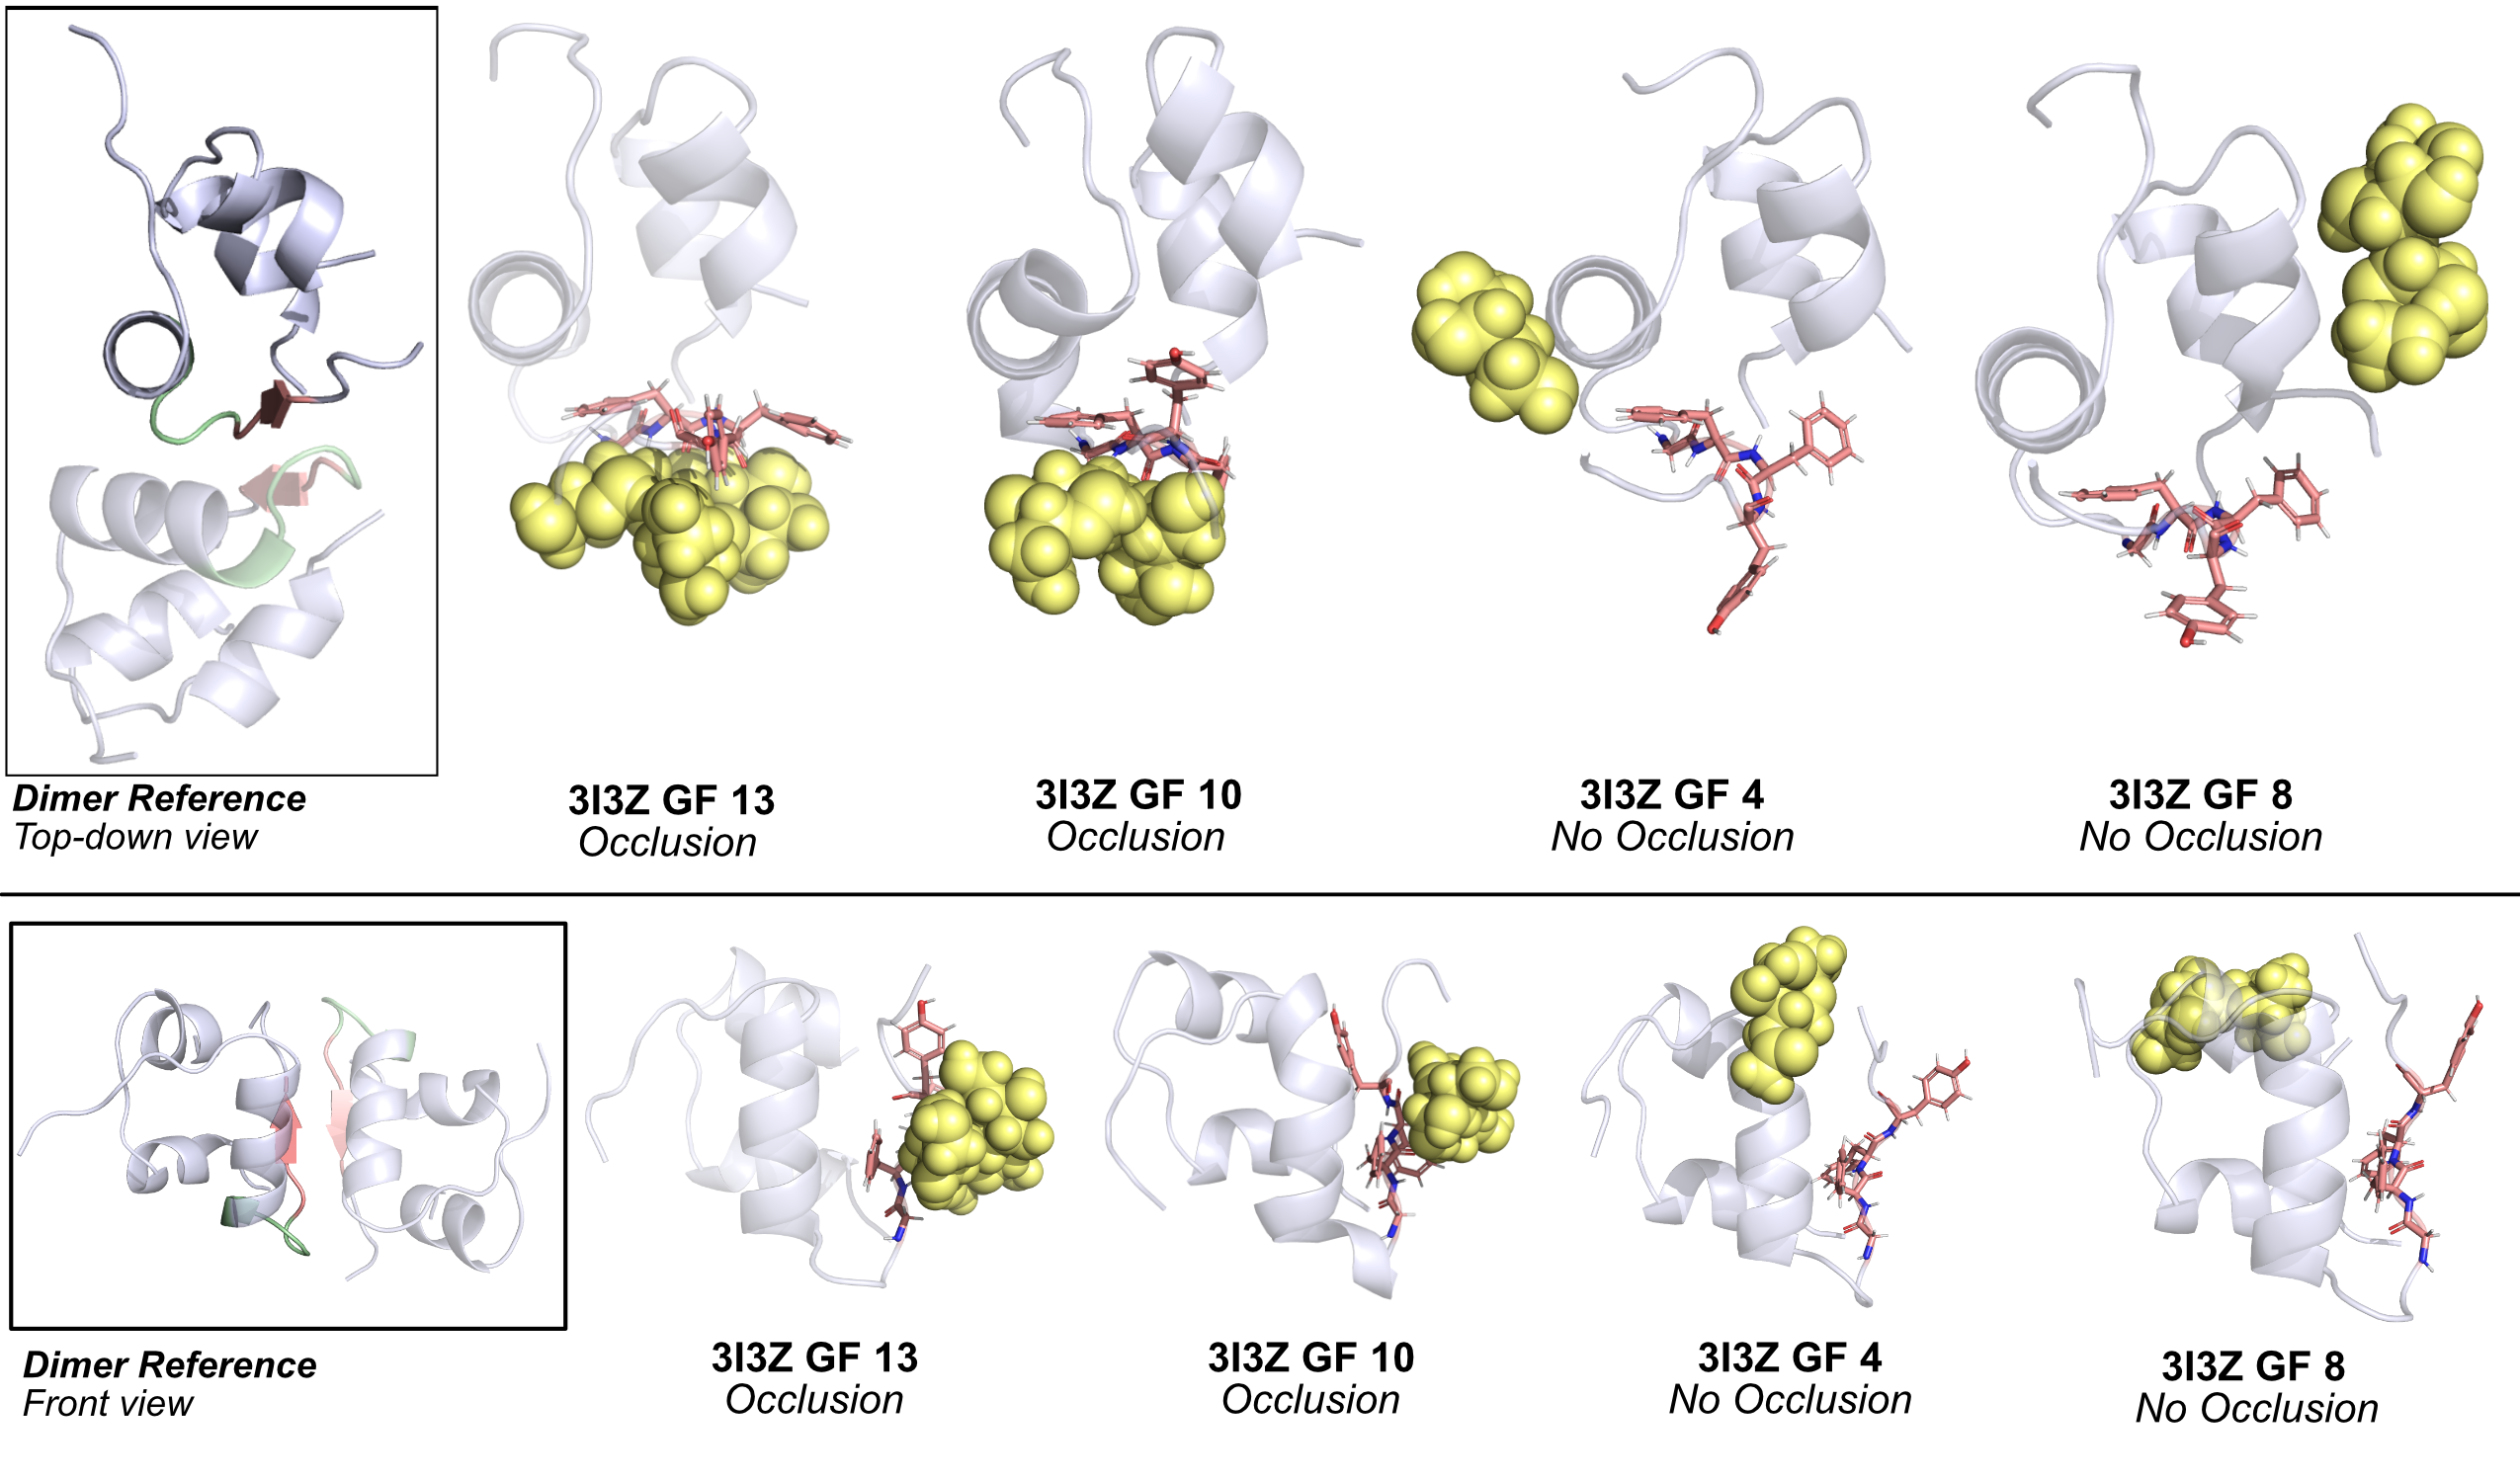
\includegraphics[width=\textwidth]{Figures/Fig_dimer_occlusion.png}
\caption{Classification of occlusion and no-occlusion states. Representative frames from four different glycoform trajectories show occlusion (GF 13, GF 10) and no occlusion (GF 4, GF 8) states. Insulin monomer \DIFaddbeginFL \DIFaddFL{is }\DIFaddendFL presented in translucent blue-white cartoon, dimerization residues presented in salmon sticks, and glycan moiety presented in yellow spheres. \DIFaddbeginFL \DIFaddFL{The 3I3Z dimer structure is provided as the reference.}\DIFaddendFL }
\label{occlusion}
\end{figure}

\DIFaddbegin \subsection{\DIFadd{Bootstrap methods for estimating the uncertainties of correlation coefficients}} \label{bootstrap}
\DIFadd{In the correlation plots presented in both the main text and the supporting information, we performed bootstrapping to estimate the uncertainties of correlation coefficients. 
}

\DIFadd{Specifically, in the main text, all the correlation plots characterize the relationship between one metric and the experimental data. Therefore, in each of the 500 bootstrap iterations we performed, for each variant, we drew five bootstrap samples for value of the metric from the set of five different wild-type models, and five bootstrap samples for the experimental reference from normal distributions centered at the experimental values. From each of these 500 bootstrap iterations, we calculated one Kendall's tau correlation coefficient by correlating the sample mean of the two variables. Lastly, we calculated the standard deviation of these 500 values and reported it as the uncertainty of the correlation coefficient. 
}

\DIFadd{The same bootstrap method was used to estimate the uncertainty of the Pearson correlation coefficients annotated in Supplemental Figure S3 to S5, except that the bootstrap samples for both metric variables of interest were drawn from values based on different wild-type models.
}

\DIFaddend \subsection{Molecular Visualization}
Molecular visualization, specifically for Figure \ref{sys_of_interest}, \ref{starting_structures}, \DIFaddbegin \DIFadd{\ref{P_sites}, }\DIFaddend \ref{occlusion}, and \DIFdelbegin \DIFdel{S1}\DIFdelend \DIFaddbegin \DIFadd{S6}\DIFaddend , were done using PyMOL version 2.4.1~\cite{delano2002pymol}.

%DIF <  \begin{itemize}
%DIF <      \item \st{Only considering monomer vs. dimer since insulin has to dimerize before it can oligomerize.}
%DIF <      \item \st{Focus on residues B17-26.}
%DIF <      \begin{itemize}
%DIF <          \item \st{This encompasses the entire dimerization interface (B23-26) and extra residues (B17-22) which I hypothesized had a different structure based on whether in the dimer or monomer}
%DIF <          \item \st{See here in the research journal for citations for the dimer interface} 
%DIF <      \end{itemize}   
%DIF <      \item Observable: dimerization by DSSP
%DIF <      \begin{itemize}
%DIF <          \item Hypothesis: Region B17-26 becomes more helical in the dimer-favored structure vs. monomer favored structure.
%DIF <          \item \st{Method: DSSP calculations for every time frame to determine the secondary structure assignments for the residues of interest}
%DIF <          \item \st{Method: Calculate autocorrelation time for each of the DSSP assignments to determine the lag-time and subsequent sample size for each of the assignments}
%DIF <          \item Analysis/prediction metric
%DIF <          \begin{itemize}
%DIF <              \item More DSSP helix assignment = more dimer propensity
%DIF <              \item Baseline = helix assignment for corresponding WT model
%DIF <          \end{itemize}
%DIF <          \item Drawback/potential criticism
%DIF <          \begin{itemize}
%DIF <              \item Differences in dssp are small, without strong signal:noise the prediction is uncertain between glycoforms
%DIF <              \item Autocorrelation of helix assignment poses problem for statistical certainty (small sample sizes)
%DIF <          \end{itemize}       
%DIF <      \end{itemize}
%DIF <      \item Observable: dimerization by glycan-interface interactions
%DIF <      \begin{itemize}
%DIF <          \item Description of figure: image illustrating where the dimer interface residues are, and the type of interactions necessary/possible for dimerization
%DIF <          \item Hypothesis: Interactions between glycan and dimer interface suggest steric occlusion, which will prevent insulin dimerization.
%DIF <          \item Method: calculate the number of neighbors (atom in glycan -- atom in interface) within 5.0A throughout simulation and for each time frame treat as binary (1 = at least one neighbor interaction present; 0 = no neighbor interaction present)
%DIF <          \begin{itemize}
%DIF <              \item Reason for this -- used binary outcome to reduce neighbor space in analysis; larger glycans will have more neighbors by default but doesn’t necessarily mean it will occlude better than smaller glycans; any interaction is possible occlusion
%DIF <          \end{itemize}
%DIF <          \item Method: Calculate autocorrelation time of the number of neighbor interactions to determine lag-time and subsequent sample size for neighbor interactions
%DIF <          \item Analysis/prediction metric
%DIF <          \begin{itemize}
%DIF <              \item More proportion time frames with glycan-interaction/occlusion = less dimer propensity
%DIF <          \end{itemize}
%DIF <          \item Drawback/potential criticism:
%DIF <          \begin{itemize}
%DIF <              \item There is no negative control i.e. no way to compare to wild-type insulin
%DIF <              \item Cannot assess percentage of dimerization relative to wild-type.
%DIF <          \end{itemize}
%DIF <      \end{itemize}
%DIF <  \end{itemize}   
\DIFdelbegin %DIFDELCMD < 

%DIFDELCMD < %%%
\DIFdelend % %===============================
% % Results and Discussions
% %===============================
\section{Results and Discussions}\label{results}
\subsection{Proteolytic degradation}
\paragraph{Metric 1: SASA of scissile bonds}
According to our hypothesis of the peptide bond SASA of the cleavage sites, glycoforms whose scissile bonds are less solvent-exposed should have higher proteolytic stability. To examine this hypothesis, we plotted the $\alpha$-chymotrypsin half-life measured in the experimental work against the SASA value of each of the two scissile bonds, including the one between residues B25 and B26 (upper panel of Figure \ref{result_sasa}A) and the one between residues B26 and B27 (lower panel of Figure \ref{result_sasa}A). Ideally, a good computational metric should be able to reproduce consistent results as compared to the work by Guan et al.~\cite{guan2018chemically}, leading to a Kendall's tau correlation coefficient close to -1. A good metric should also be immune to the starting model bias, including the bias from wild-type models resolved using different methods or under different conditions, or the bias solely from different protonation states of the histidine residues. 

As a result, we \DIFdelbegin \DIFdel{concluded that although }\DIFdelend \DIFaddbegin \DIFadd{conclude that }\DIFaddend the SASA of the scissile bonds \DIFdelbegin \DIFdel{was free from inital structure bias, it was only }\DIFdelend \DIFaddbegin \DIFadd{is }\DIFaddend a weak predictor for proteolytic stability. GF 13 and GF 10, which were experimentally found to be more proteolytically stable than the wild type, did have a lower SASA value than the wild type at both sites. Notably, as the most proteolytically stable structure, GF 13 also had the lowest SASA values at both sites. However, GF 10 had the second-longest $\alpha$-chymotrypsin half-life, but not the second-lowest SASA values at both sites. At the scissile bond between B26 and B27, most glycoforms had a lower SASA value than that of the wild type, but some of them were experimentally identified as less proteolytically stable than the wild type. Overall, the SASA values of either scissile bond have roughly the same efficacy given similar values of Kendall\DIFdelbegin \DIFdel{'}\DIFdelend \DIFaddbegin \DIFadd{’}\DIFaddend s tau correlation coefficients. However, if we are only interested in the comparison between the wild type and any glycoform instead of between any two of the glycoforms, the SASA value of the scissile bond between B25 and B26 is marginally more indicative than the SASA value of the other site. \DIFdelbegin \DIFdel{For glycoforms having lower permeability }\DIFdelend \DIFaddbegin \DIFadd{Specifically, among all the glycoforms that had shorter $\alpha$-chymotrypsin half-lives }\DIFaddend than the wild type, \DIFdelbegin \DIFdel{such as }\DIFdelend GF 3, GF 4, GF 7, and GF 8 \DIFdelbegin \DIFdel{, the SASA values were indeed higher than the wild type. Still, some of its predictions provided opposite results as compared to the experimental ones (}\DIFdelend \DIFaddbegin \DIFadd{indeed had higher SASA values at this site than the wildtype. As for }\DIFaddend GF 6 and GF 11\DIFdelbegin \DIFdel{). Importantly, all observations are independent of different initial wild-type structures, which is reflected by the small error bars of the SASA values}\DIFdelend \DIFaddbegin \DIFadd{, which also had short $\alpha$-chymotrypsin half-lives than the wild type, the SASA value at the B25-B26 scissile bond failed to classify them as the less proteolytically stable variants. Notably, the errors in the metric are generally large, which might be attributable to the fact that the SASA of the scissile bond was calculated from only 4 atoms (CONH atoms) and could lead to larger fluctuations in nature. Regardless of whether these large error bars are a direct result of the dependence of the initial bias or not, this high uncertainty undermined the predictiveness of this metric, making it less useful}\DIFaddend .

\begin{figure}[H]
\centering
\DIFdelbeginFL %DIFDELCMD < \includegraphics[width=\textwidth]{Figures/Figure4.png}
%DIFDELCMD < %%%
\DIFdelendFL \DIFaddbeginFL 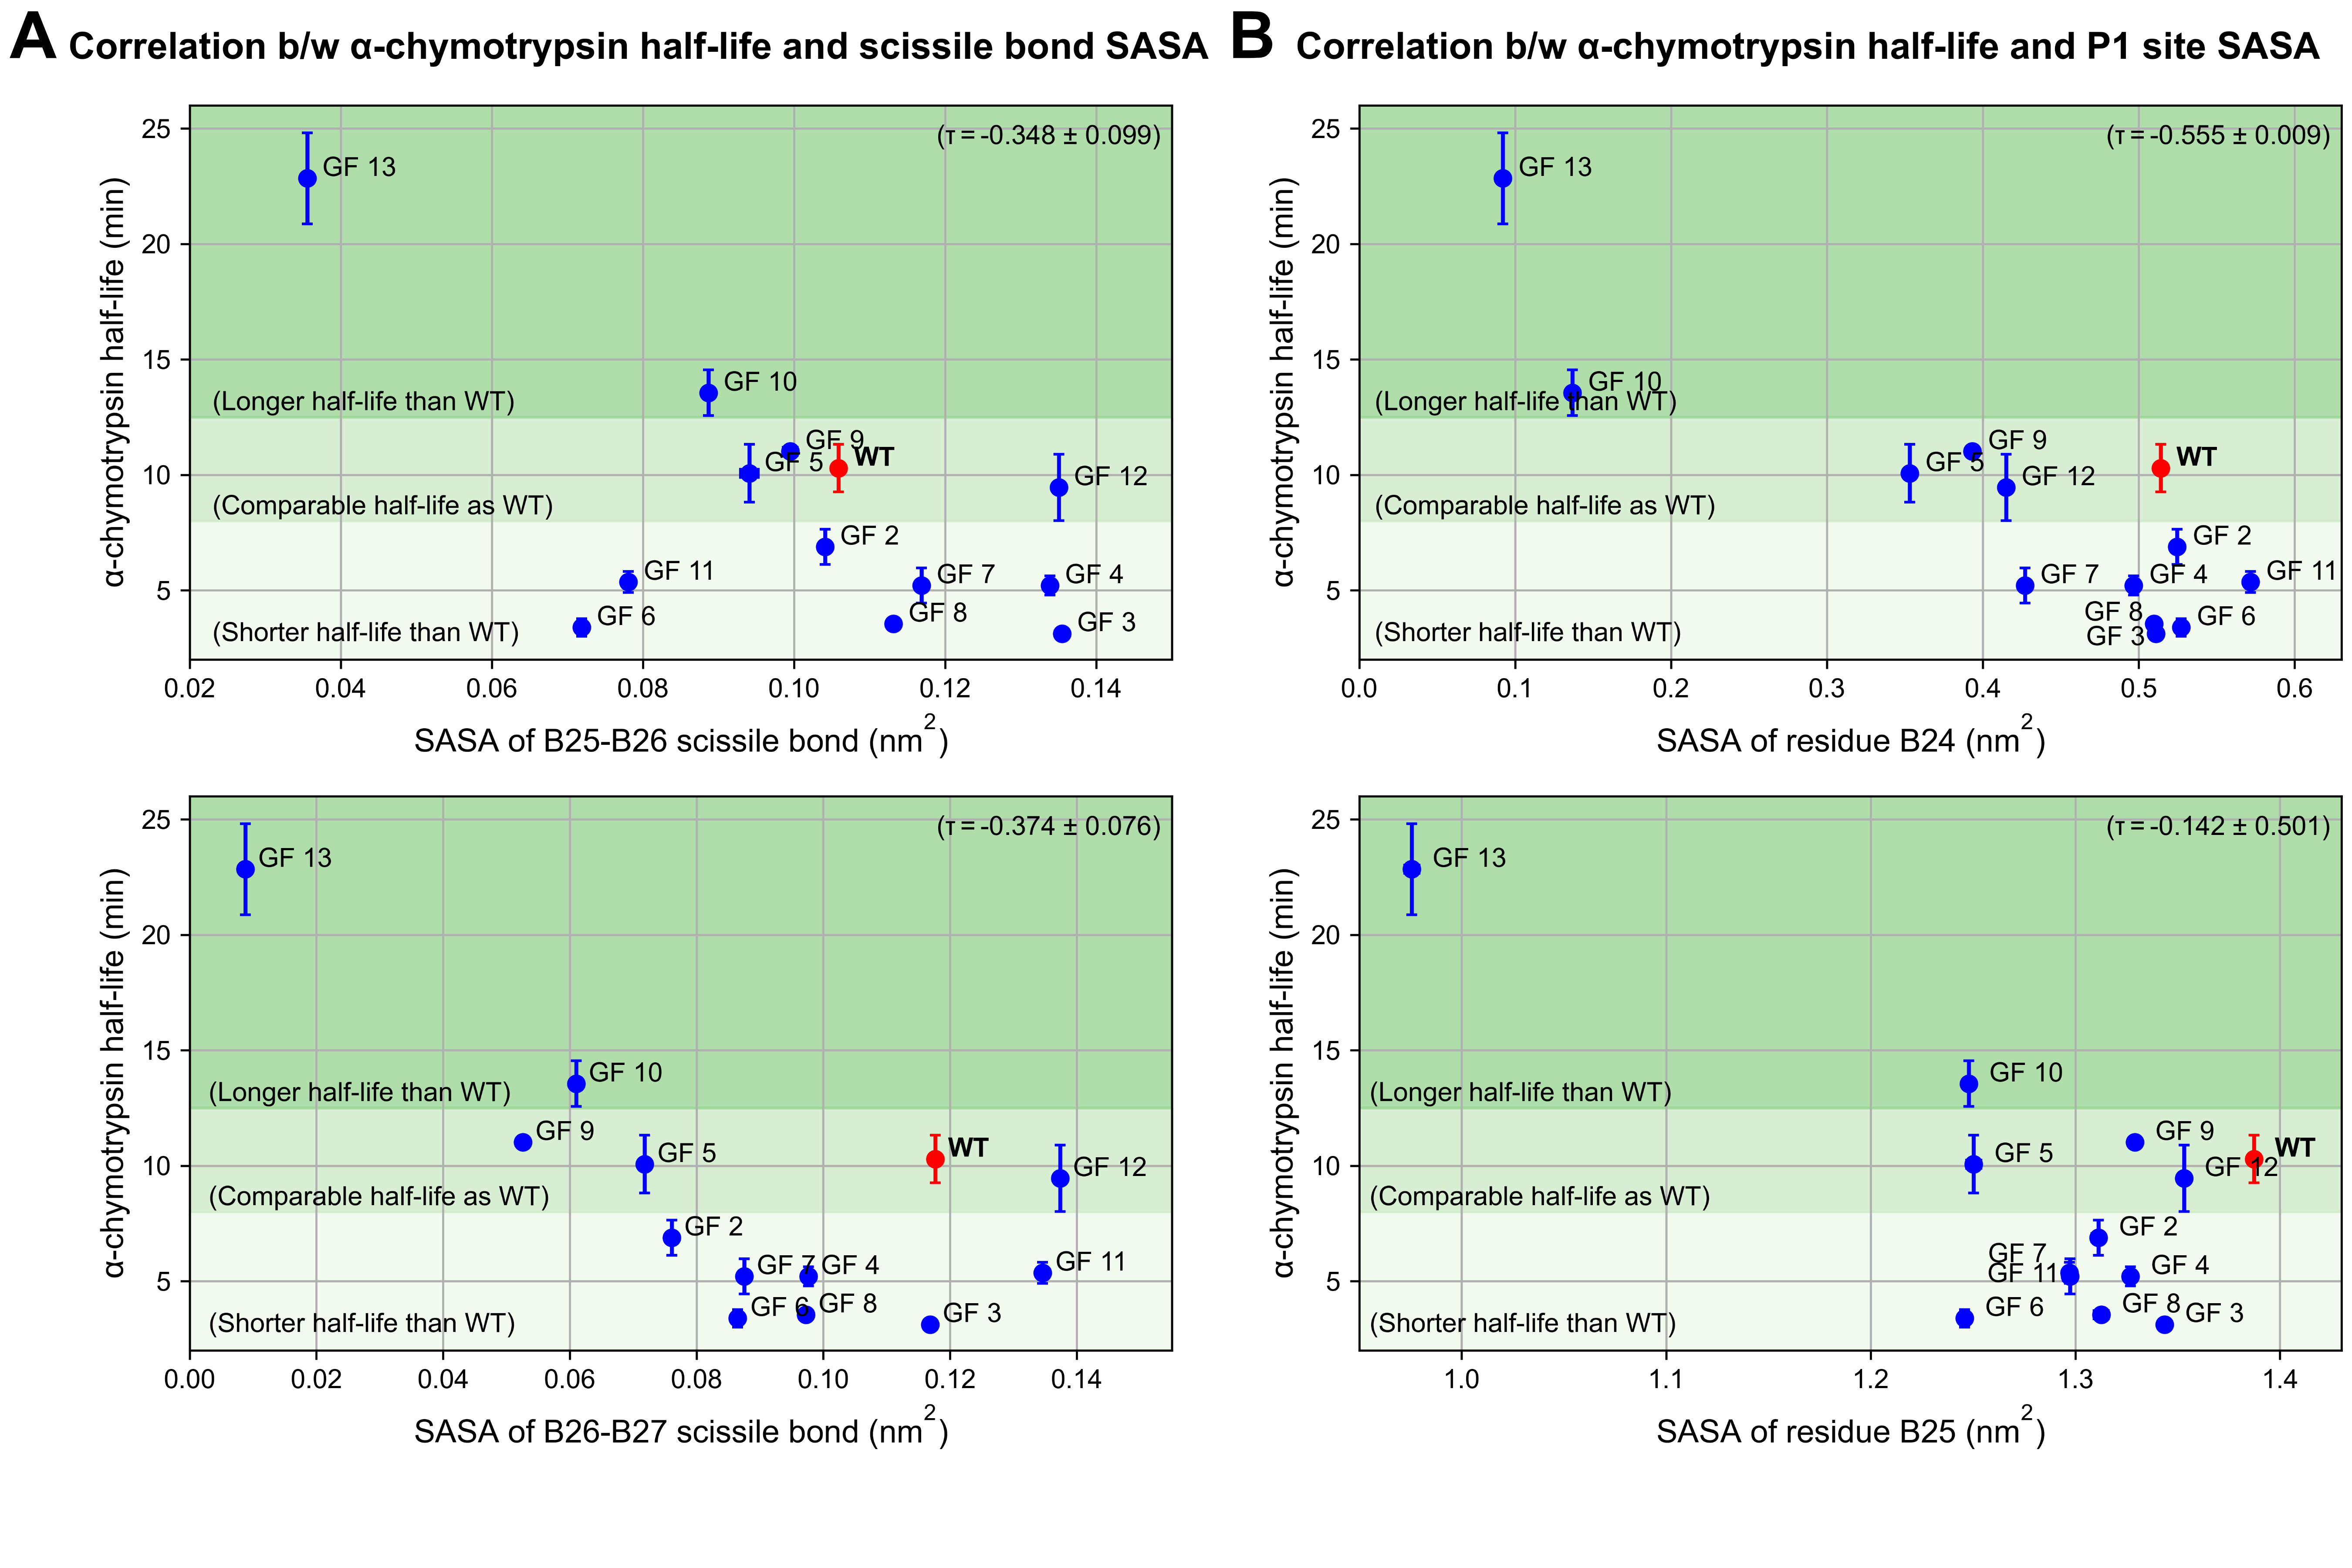
\includegraphics[width=\textwidth]{Figures/Fig_SASA_correlation.png}
\DIFaddendFL \caption{The SASA of both the scissile bonds and the P1 sites are weakly correlated with $\alpha$-chymotrypsin half-life, implying moderate \DIFdelbeginFL \DIFdelFL{predicitveness }\DIFdelendFL \DIFaddbeginFL \DIFaddFL{predictiveness }\DIFaddendFL for the proteolytic stability. (A) The correlation plot between the $\alpha$-chymotrypsin half-life and the average SASA of the scissile bonds in the glycoforms (GF). (B) The correlation plot between the $\alpha$-chymotrypsin half-life and the average SASA of the P1 sites in the glycoform (GF). Different regions were colored to indicate glycoforms having longer, comparable\DIFaddbeginFL \DIFaddFL{, }\DIFaddendFL or shorter half-life as compared with the wild type. The Kendall's tau correlation coefficient ($\tau$) and its \DIFdelbeginFL \DIFdelFL{two-tailed p-value }\DIFdelendFL \DIFaddbeginFL \DIFaddFL{uncertainty }\DIFaddendFL were calculated. Error bars of both variables are shown\DIFdelbeginFL \DIFdelFL{, but the error bars }\DIFdelendFL \DIFaddbeginFL \DIFaddFL{. The distributions }\DIFaddendFL of the \DIFdelbeginFL \DIFdelFL{SASA metrics }\DIFdelendFL \DIFaddbeginFL \DIFaddFL{data }\DIFaddendFL are \DIFdelbeginFL \DIFdelFL{generally very small and invisible}\DIFdelendFL \DIFaddbeginFL \DIFaddFL{provided in Supplemental Figure S2}\DIFaddendFL .}
\label{result_sasa}
\end{figure}

\paragraph{Metric 2: SASA of the P1 sites}
\DIFdelbegin \DIFdel{Similarly }\DIFdelend \DIFaddbegin \DIFadd{Similar }\DIFaddend to Metric 1, Metric 2 is \DIFdelbegin \DIFdel{independent of the initial wild-type structures, as evidenced by the small error bars of the SASA values. 
However, we again concluded that it was partially predictive. 
}\DIFdelend \DIFaddbegin \DIFadd{partially predictive and has relatively large error bars for some of the variants. 
}\DIFaddend 

In the lower panel of Figure \ref{result_sasa}B, the SASA of residue B25 is less predictive than the SASA of the other site. Although \DIFaddbegin \DIFadd{an }\DIFaddend agreement with experimental results can be seen from GF 13, which had the lowest SASA at residue B25 and was previously found to be the most proteolytically stable, other glycoforms, regardless of the $\alpha$-chymotrypsin half-life, all had a lower value compared to the wild type. The \DIFdelbegin \DIFdel{Kandall}\DIFdelend \DIFaddbegin \DIFadd{Kendall}\DIFaddend 's tau correlation coefficient, which was close to 0, \DIFdelbegin \DIFdel{showing }\DIFdelend \DIFaddbegin \DIFadd{shows }\DIFaddend that the SASA of residue B25 was almost uncorrelated with the $\alpha$-chymotrypsin half-life. 

The SASA of residue B24 (the upper panel of Figure \ref{result_sasa}B), on the other hand, had a higher correlation with the proteolytic stability of the structure. Specifically, GF 13 and GF 10, the two most proteolytically stable glycoforms, had significantly lower SASA value at residue B24. As for the glycoforms that had a lower SASA value at this site, except for GF 7, all had comparable proteolytic stability to the wild type. This higher correlation can also be seen from the magnitude of the corresponding Kendall's tau correlation coefficient, which was higher than those of Metric 1.

Overall, these observations imply moderate predictiveness of the SASA of residue B24, since a low value at this site generally indicates that the structure is very likely to have more, or at least comparable proteolytic stability compared to the wild type. Notably, most proteolytically unstable glycoforms, including GF 2, GF 3, GF 4, GF 6, GF 7, and GF8, had the same level of SASA at residue B24 as the wild type. This could be attributable to the situation where the residue of the wild type is already very solvent-exposed, leaving considerably less space for the proteolytically unstable glycoforms to have an even higher SASA value. This limitation is intrinsic to both Metric 1 and Metric 2, motivating us to look for more reliable predictors for proteolytic stability. 

\paragraph{Metric 3: $\beta$-sheet propensity of the P1--P3 region}
Our hypothesis suggests that glycoforms whose P1--P3 region has a lower $\beta$-sheet propensity should potentially have higher proteolytic stability. However, \DIFdelbegin \DIFdel{from Figure~\ref{result_beta}, it can be seen that none of the examined residuesshowed this trendand all the Kendall's tau correlation coefficients were very low and highly uncertain, indicating that Metric 3 was inadequate in capturing }\DIFdelend \DIFaddbegin \DIFadd{most of the residues, including B22, B23, and B24 did not show this trend, while residue B25 did show predictiveness of roughly the same level as Metric 1 since it showed the lowest $\beta$-sheet propensity for the most proteolytically stable structures (GF 10 and GF 13). Notably, even if one of the four residues exhibited moderate predictiveness, the generally large error bars in the $\beta$-sheet propensity undermine its usage as a metric to capture }\DIFaddend structural determinants that influenced the proteolytic stability of the structure. \DIFdelbegin \DIFdel{This is also reflected by the }\DIFdelend \DIFaddbegin \DIFadd{These }\DIFaddend large error bars in the \DIFdelbegin \DIFdel{$\beta$-sheet propensity of most of the residues of interest, including residues }\DIFdelend \DIFaddbegin \DIFadd{case of }\DIFaddend B22 \DIFdelbegin \DIFdel{, B23, and }\DIFdelend \DIFaddbegin \DIFadd{to }\DIFaddend B24 \DIFdelbegin \DIFdel{. The large error bars in $\beta$-sheet propensity }\DIFdelend \DIFaddbegin \DIFadd{also }\DIFaddend imply that the structure at these sites \DIFdelbegin \DIFdel{(residues B22 to B24) }\DIFdelend can adopt a wide range of orientations, contradicting our hypothesis that the glycoforms able to prevent proteolytic degradation should have common orientations at these sites due to high free energy costs of structural re-orientations or transformations. \DIFdelbegin \DIFdel{Note }\DIFdelend \DIFaddbegin \DIFadd{Similar to the first two metrics, we note }\DIFaddend that these large error bars are not necessarily the results of the starting model bias, since the $\beta$-sheet propensity was calculated from the orientations of just a few atoms, which naturally caused larger fluctuations of the results. Since the metric is insufficient to assess the proteolytic stability, whether or not the large error bars can be ascribed to the starting model bias is not relevant. 
\DIFdelbegin \DIFdel{We note the only site that showed small error bars in the $\beta$-sheet propensity was residue B25, which might be related to the unique role of residue B25 as a P1 site and a cleavage site at the same time. However, B25 essentially has high $\beta$-sheet propensity in all glycoforms, so variability at this site cannot be used.
}\DIFdelend 


\begin{figure}[H]
\centering
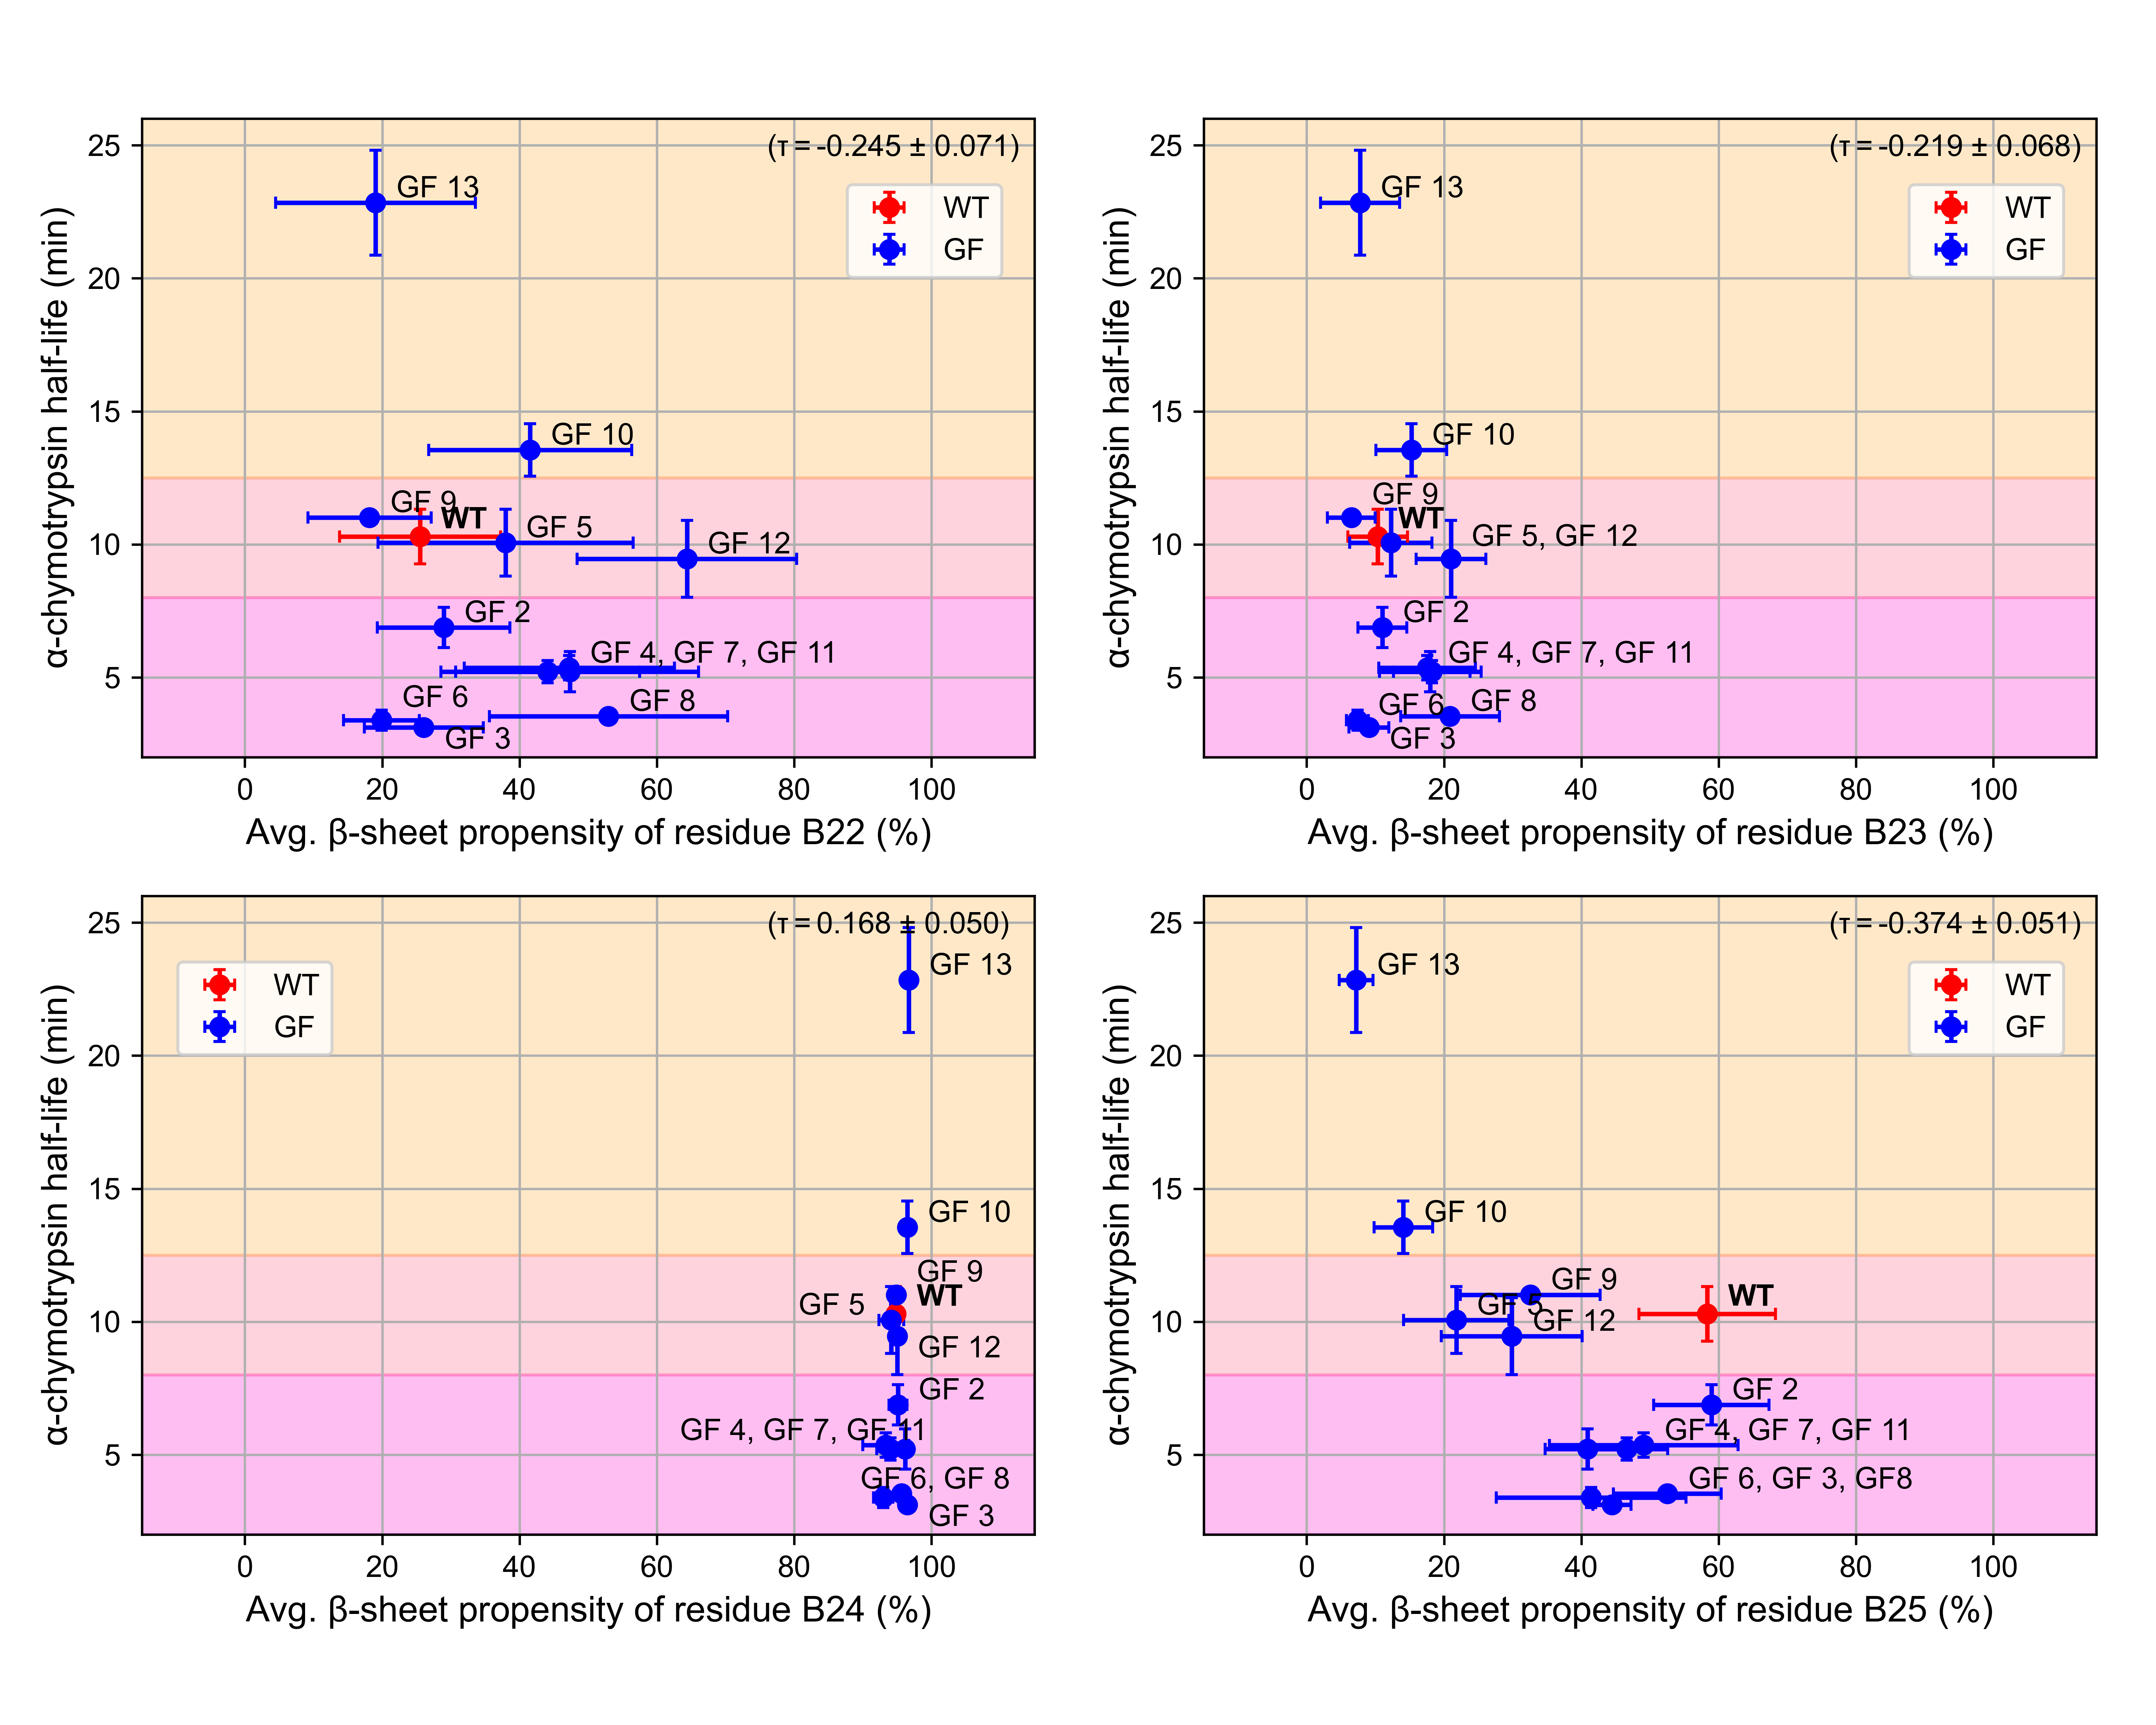
\includegraphics[width=\textwidth]{Figures/avg_beta_propensity_correlation.png}
\caption{The correlation plot between the $\alpha$-chymotrypsin half-life and the average $\beta$-sheet propensity of residues B22 to B25. The $\beta$-sheet propensity of the P1-P3 region does not correlate with $\alpha$-chymotrypsin half-life. Different regions were colored to indicate glycoforms having longer, comparable\DIFaddbeginFL \DIFaddFL{, }\DIFaddendFL or shorter half-life as compared with the wild type. The Kendall's tau correlation coefficient ($\tau$) and its \DIFdelbeginFL \DIFdelFL{two-tailed p-value }\DIFdelendFL \DIFaddbeginFL \DIFaddFL{uncertainty }\DIFaddendFL were calculated. Error bars of both variables are shown.}
\label{result_beta}
\end{figure}

\paragraph{Metric 4: Existence of glycan-involved hydrogen bonds}
We hypothesized that glycoforms with more glycan-involved hydrogen bonds, especially the ones that \DIFdelbegin \DIFdel{involve }\DIFdelend \DIFaddbegin \DIFadd{involved }\DIFaddend the P1--P3 or the P2' sites, could interfere with the canonical hydrogen-bonding network formed between the protease and the substrate, thus enhancing the proteolytic stability of the substrate. This metric does turn out to be in large part predictive of proteolytic stability of the glycoforms. 

Figure \ref{result_hbond} shows the percentage of the time each kind of hydrogen bond existed in the MD simulations. As a result, proteolytically stable glycoforms such as GF 13 and GF 10 had the most glycan-involved hydrogen bonds. Glycoforms with comparable proteolytic stability as the wild type, including GF 5, GF9, and GF 12 had at least one or two glycan-involved hydrogen bonds. Most of the remaining glycoforms, which were more susceptible to proteolytic degradation than the wild type, had no glycan-involved hydrogen bonds. Importantly, glycoforms having at least comparable proteolytic stability as the wild type typically have hydrogen bonds that involved residues PheB24 or ThrB27, which were the P1 site and the P2' site corresponding to the cleavage site B25, respectively. In glycoforms that had an intermediate level of proteolytic stability (GF 5, and GF 9), hydrogen bonds involving these two residues were not present or at least not long-lasting in the MD trajectories (see Supplemental Table \DIFdelbegin \DIFdel{S3}\DIFdelend \DIFaddbegin \DIFadd{S5}\DIFaddend ), as reflected by the large errors bars that almost reached the bottom of the graph. On the other hand, in the proteolytically stable glycoforms, GF 13 and GF 10, hydrogen bonds ThrB27(N)--Man[2](O6) and PheB24(N)--Man[1](O3) were found in all GF 13/GF 10 MD trajectories, regardless of which wild-type model the glycoform was built on. We concluded these two kinds of hydrogen bonds (ThrB27(N)--Man[2](O6) and PheB24(N)--Man[1](O3)), the longest-lasting glycan-involved hydrogen bonds in the most proteolytically stable structures, were the most important hydrogen bonds influencing the proteolytic stability in our study. Interestingly, GF 13 occasionally had a hydrogen bond formed between ThrB27 and the third mannose, which was absent from GF 10. This additional hydrogen bond that involved a P2' site might further interfere with the hydrogen bonding network between insulin and $\alpha$-chymotrypsin, making GF 13 even more proteolytically stable than GF 10. 

Overall, the predictions made out of the glycan-involved hydrogen bonds analysis are relatively consistent with the experimental results. The only exception is GF 6, which was experimentally found to be less proteolytically stable than the wild type but had a hydrogen bond, ThrB27(N)-GalNAc[1](O3) that involved a P2' site ThrB27. However, this hydrogen bond was only present in the MD trajectories of 4EYD-, 4EY1-, and 2MVC-based GF 6 (see Supplemental Table \DIFdelbegin \DIFdel{S3}\DIFdelend \DIFaddbegin \DIFadd{S5)}\DIFaddend , indicating that this hydrogen bond might not be stable enough to consistently disturb the aforementioned hydrogen bonding network. Importantly, the fact that 4EYD-, 4EY1-, and 2MVC-based GF 6 all possess the same hydrogen bond is one of many examples showing the large error bars should be irrelevant to the initial modeling bias. Specifically, if there is a bias from the differences in the resolution methods or the histidine protonation states, glycoforms resolved by the same method (e.g. 4EYD-, 4EY9-, and 4EY1-based glycoforms) or having the same histidine protonation states (e.g. 4EYD-, 4EY1- and 3I3Z-based glycoforms) should exhibit similar hydrogen bond distributions at the examined site. However, this trend is absent from our results, suggesting that the metric is independent of the starting wild-type models. Finally, we can conclude that long-lasting, stable glycan-involved hydrogen bonds, especially the ones that involve PheB24 and ThrB27, appear critical in enhancing the proteolytic stability of the structure. This conclusion also \DIFdelbegin \DIFdel{upderpins }\DIFdelend \DIFaddbegin \DIFadd{underpins }\DIFaddend the findings in the work by Guan et al.~\cite{guan2018chemically} that ThrB27 and ThrB30 were identified as the best two glycosylation sites, as the glycan attached to these sites are structurally closer to the important residues (ThrB27 and PheB24) found in this study. 
\begin{figure}[H]
\centering
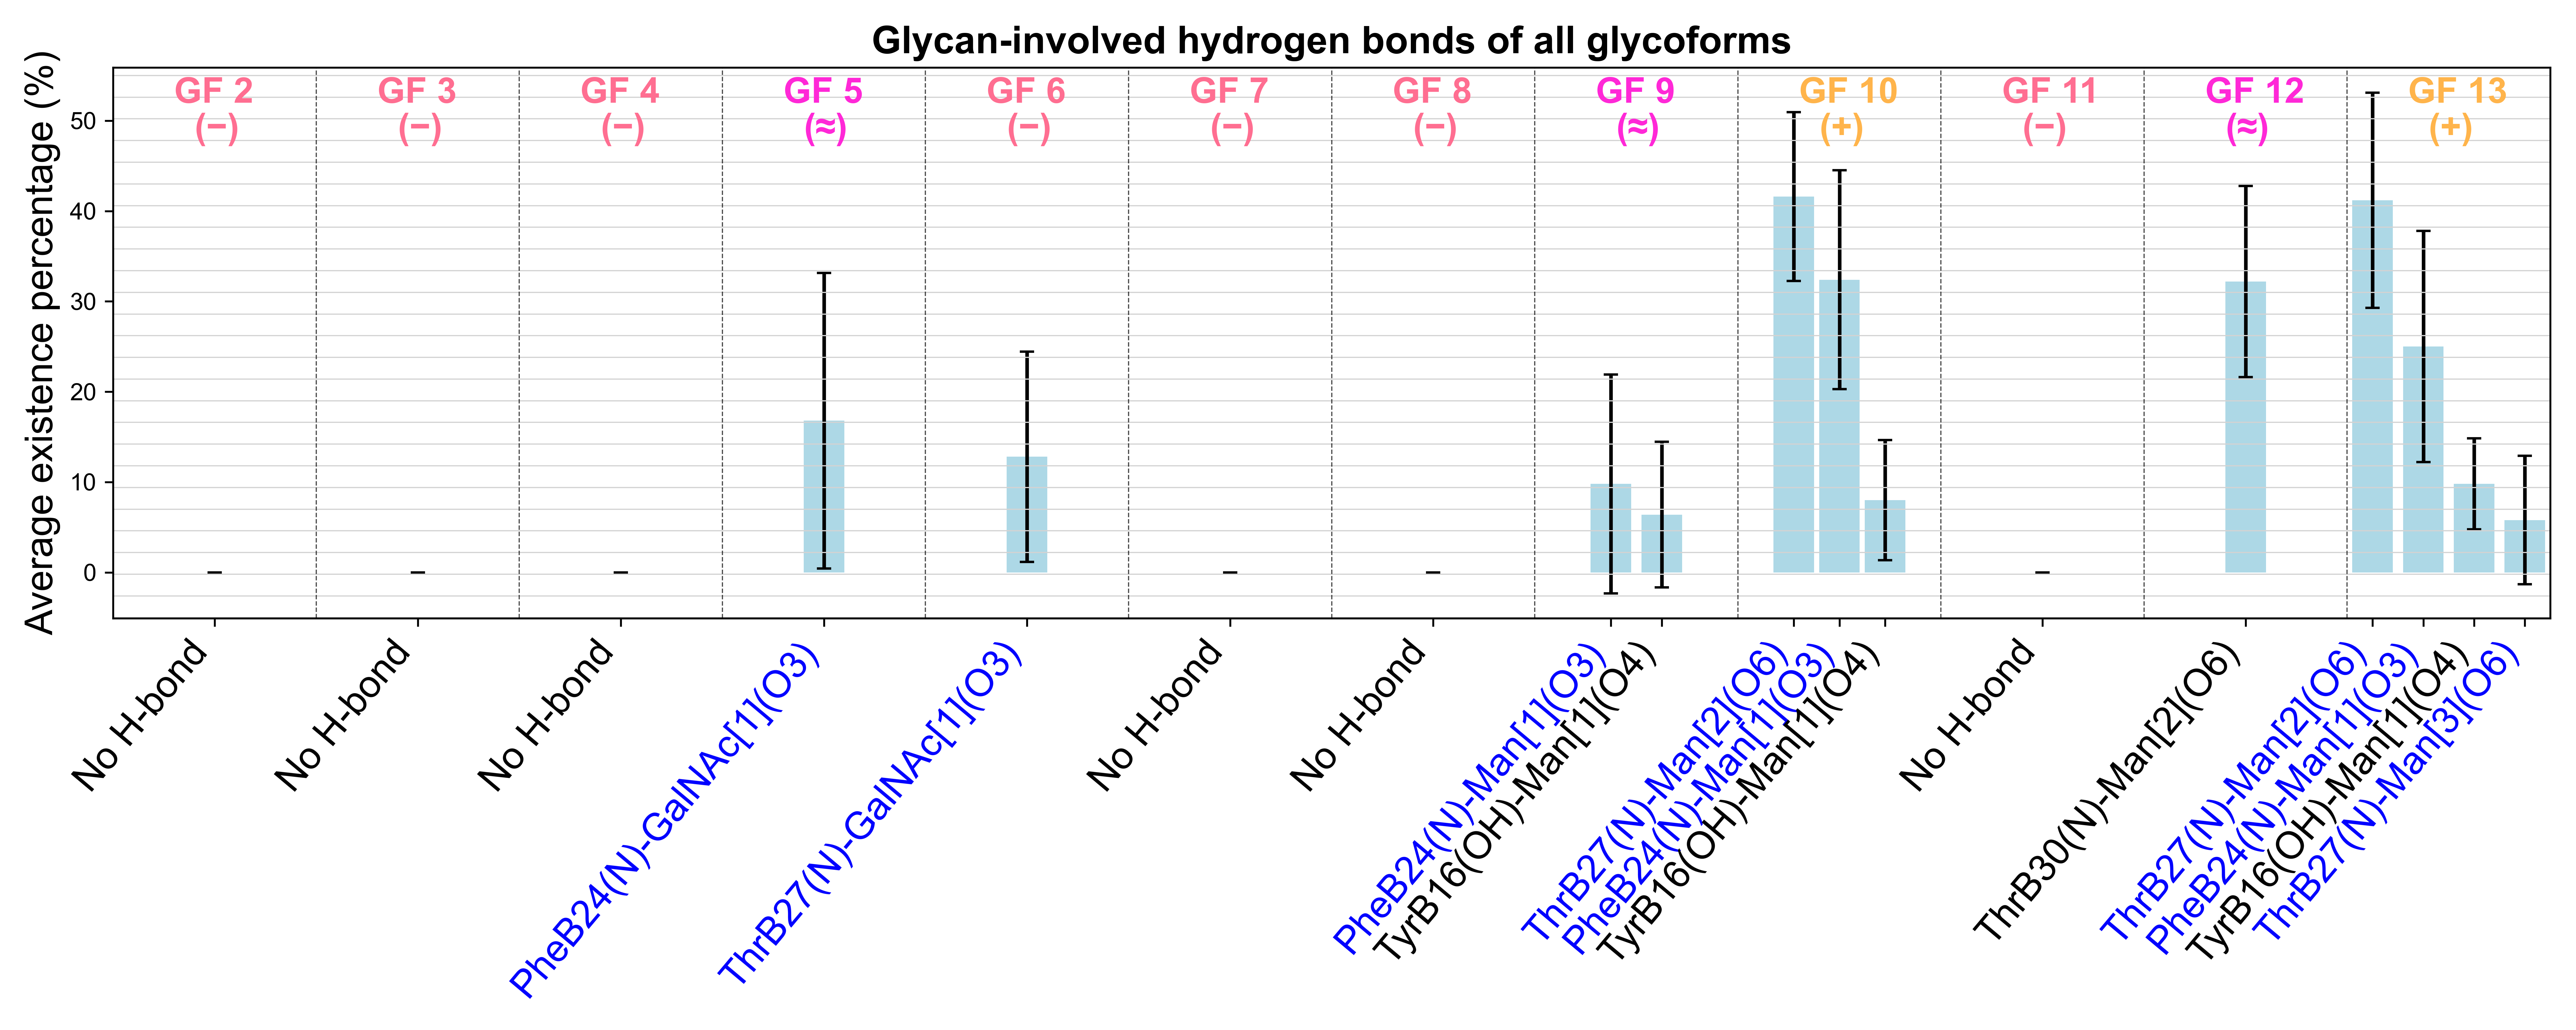
\includegraphics[width=\textwidth]{Figures/hbond_results.png}
\caption{The most proteolytically stable glycoforms tend to have more glycan-involved hydrogen bonds, especially the ones involving the residues PheB24 and ThrB27. The figure shows the \DIFdelbeginFL \DIFdelFL{average }\DIFdelendFL percentage of the time \DIFdelbeginFL \DIFdelFL{of }\DIFdelendFL each \DIFaddbeginFL \DIFaddFL{kind of }\DIFaddendFL hydrogen bond existed in the MD simulations. The experimental results are summarized such that $+$(yellow), $-$(red), and $\approx$(magenta) respectively indicate that the corresponding glycoform was experimentally found to have higher, lower and comparable proteolytic stability as compared to the wild type. Note that in the name of each hydrogen bond, the 1-based index of the glycan is shown in the bracket following the name of the glycan. The atom type is shown in the parenthesis right after the residue name. (See Supplemental Table \DIFdelbeginFL \DIFdelFL{S4 }\DIFdelendFL \DIFaddbeginFL \DIFaddFL{S6 }\DIFaddendFL for more details of the atom types shown in the figure.) For example, ThrB27(N)--Man[2](O6) means the hydrogen bond formed between the amide N atom of ThrB27 as the donor and one of the oxygen atoms of the second mannose as the acceptor. \DIFdelbeginFL \DIFdelFL{Text }\DIFdelendFL \DIFaddbeginFL \DIFaddFL{Texts }\DIFaddendFL for hydrogen bonds that involve any of the P1--P3 or the P2' residues are colored in blue, which in our case only include PheB24 and ThrB27.}
\label{result_hbond}
\end{figure}

%DIF < \begin{itemize}
%DIF <     \item \st{Should mention that the results are independent of the initial model of human insulin.}
%DIF <     \item \st{Should mention that the protontation states did not influence the results of each method.} 
%DIF <     \item \st{SASA of the proteolyic cleavage sites is not useful to understand susceptibility to degradation}
%DIF <     \item \st{Ramachandran plots looking at propensity to be in the transition state is not useful.}
%DIF <     \item \st{H-bond analysis is useful.}
%DIF <     \begin{itemize}
%DIF <         \item \st{Hydrogen bonds formed between the glycan and the residues PheB24 or ThrB27 are found to be important in enhancing the proteolytic stability of the structure. }
%DIF <         \item \st{In glycoforms where the sugar is a monomer, the hydrogen bond PheB24(N)--Sugar52(O3) can potentially make the structure more proteolytically stable.}
%DIF <         \item \st{For glycoforms where the sugar is a mannose dimer or} 
%DIF <         \item \st{Description of Fig X,YZ.}
%DIF <         \item \st{Figure: what an h-bond pattern is that is likely to interfere with things.}
%DIF <     \end{itemize}
%DIF < \end{itemize}       
\DIFdelbegin %DIFDELCMD < 

%DIFDELCMD < %%%
\DIFdelend \subsection{Dimerization Propensity}
\paragraph{Metric 1: Glycan-dimer occlusion}
Based on our dimerization hypothesis, glycoforms whose glycans come in proximity to the dimer interface (GlyB23--PheB26) will be less prone to dimerize because of steric occlusion by the glycan. We found that this glycan-dimer occlusion might be a useful predictor of dimerization propensity. 

To test this hypothesis, we calculated the glycan-dimer occlusion metric for each glycoform and considered those with low occlusion to have high dimerization propensity, and vice versa. Figure~\ref{occlusion} shows representative frames from four 3I3Z trajectories to visually demonstrate occlusion versus no-occlusion, where the light blue cartoon represents insulin, salmon sticks represent residues GlyB23--PheB26, and pale yellow spheres represent the glycan moiety. 

Using the glycan-dimer occlusion metric, we calculated the proportion of simulation frames with occlusion for each glycoform and ordered them from least occlusion to most occlusion, shown in Supplemental Table \DIFdelbegin \DIFdel{S5}\DIFdelend \DIFaddbegin \DIFadd{S7}\DIFaddend . We must carefully compare these results to experimental dimerization data~\cite{guan2018chemically} because this analysis method cannot include the respective wild-type models for reference (which by default have no occlusion), which is a drawback of this metric.

There is \DIFaddbegin \DIFadd{an }\DIFaddend agreement in the order of glycoforms between model sets for this metric. While there are slight variations in the precise order between models, there are trends that sort the glycoforms into \emph{low} (GF 2, GF 3, GF 7, GF 8), \emph{medium} (GF 4, GF 6, GF 11, GF 12), and \emph{high} (GF 5, GF 9, GF 10, GF 13) occlusion batches which are independent of starting structure. This analysis consistently predicts GF 9, GF 10, and GF 13 as having the most occlusion, and therefore least dimer propensity, of the glycoforms. This is in agreement with experimental data that these glycoforms form dimers less frequently than wild-type insulin~\cite{guan2018chemically}. None of the models accurately reproduced the correct experimental dimerization order, however (GF 10 > GF 13 > GF 9).

% Talk about the proportion of occlusion, show a table, and then 
The proportion of frames with occlusion, and the associated uncertainty, were compared between glycoforms for each model (Supplemental Figure \DIFdelbegin \DIFdel{S3}\DIFdelend \DIFaddbegin \DIFadd{S7}\DIFaddend ). The Wilson score 95\% confidence intervals for each proportion is shown in red and calculated from the occlusion autocorrelation lag times, which were used to estimate the number of independent occlusion configurations sampled. Differences in occlusion proportions, particularly between the low occlusion batch and the high occlusion batch, are statistically distinguishable and this finding is true for all 5 model sets. Differences within occlusion batches are not statistically differentiable.

\begin{figure}[H]
\centering
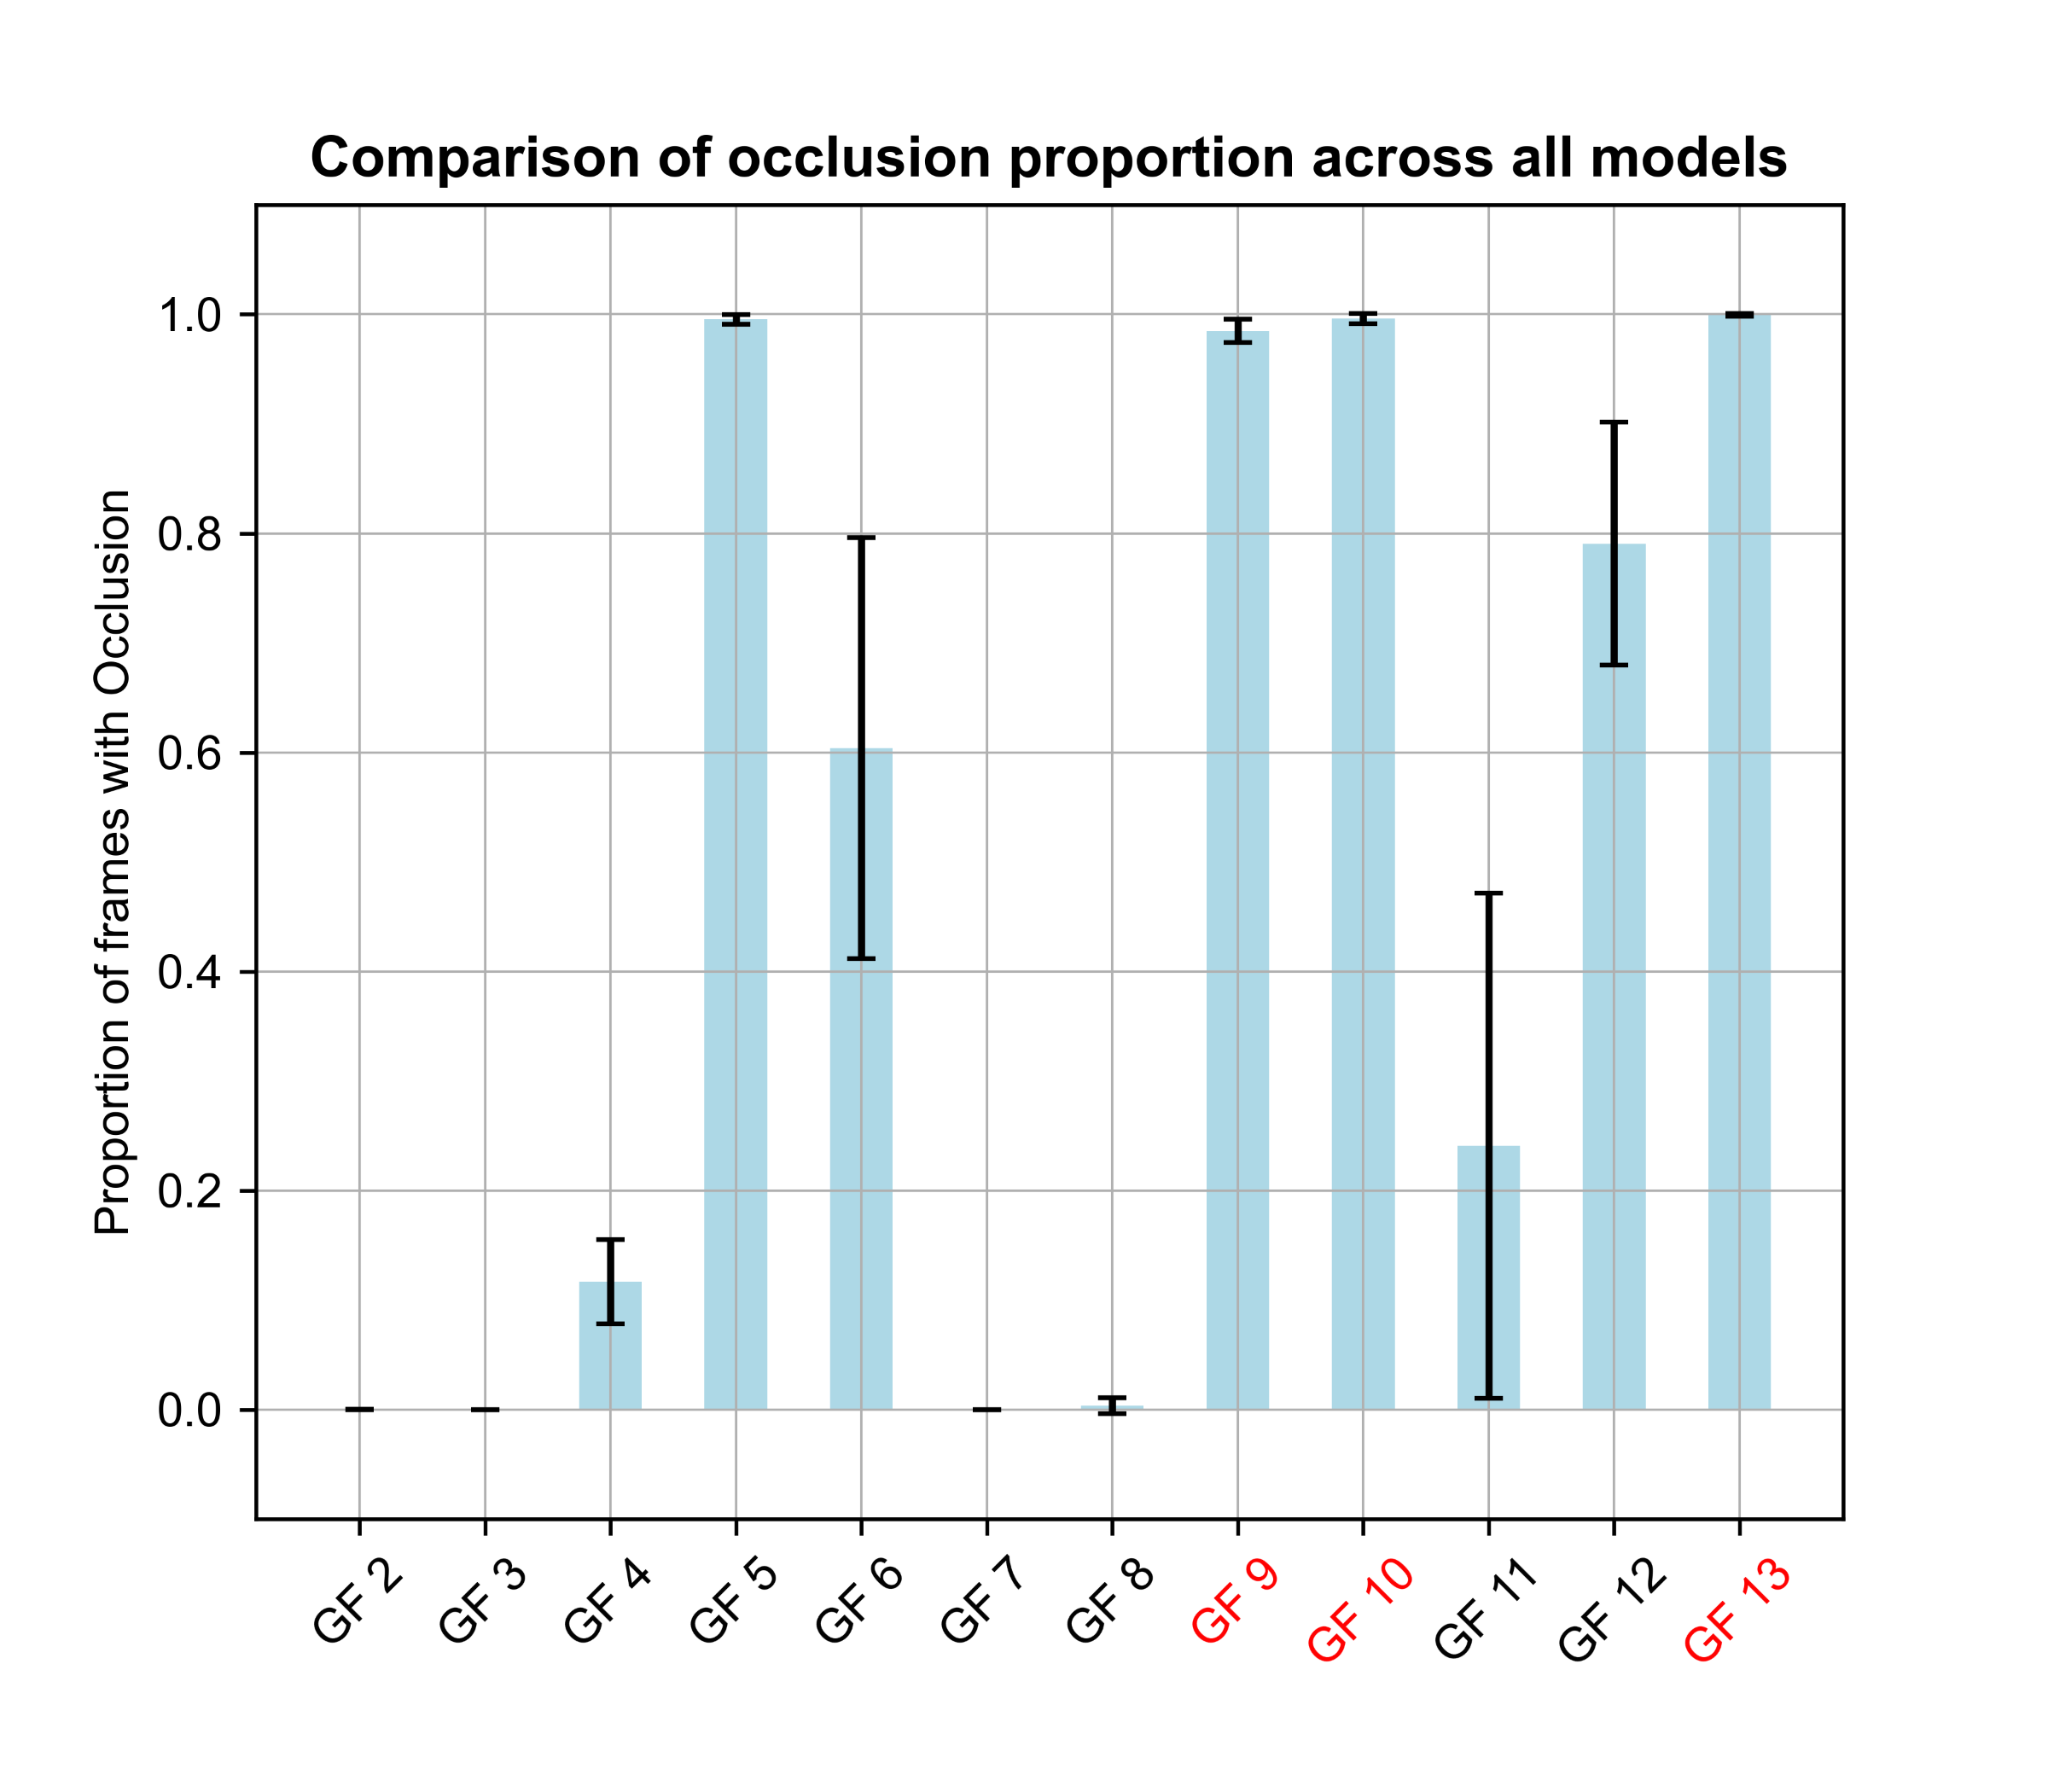
\includegraphics[width=0.50\textwidth]{Figures/occlusion_proportion_averaged.png}
\caption{Average occlusion analysis distinguishes glycoforms with low, medium, and high occlusion proportion. All five models for each glycoform were averaged for occlusion \DIFdelbeginFL \DIFdelFL{proportion}\DIFdelendFL \DIFaddbeginFL \DIFaddFL{proportions}\DIFaddendFL , and are plotted with standard deviation represented in black bars. Axis labels in red indicate glycoforms with experimental dimerization data.}
\label{occlusion_results}
\end{figure}

% Talk about independence of model
To assess the dependence of these results on the starting structural model, for each glycoform we averaged the proportion of frames with occlusion across the five models and compared the means and associated standard deviations (Figure \ref{occlusion_results}). Occlusion proportions are consistent across the models for almost all the glycoforms, particularly those in the low and high occlusion batches. There is considerable variability in the glycoforms of the medium occlusion batch (GF 6, GF 11) but considering the consistency in the other models, this might result more from initial glycoform minimization/optimization than the model itself.

% Final thoughts about the occlusion
These results suggest that the dimer occlusion metric is independent of the initial model of human insulin. Since we cannot include a wild type in this analysis, there is no negative control for each glycoform set nor is there a way to predict percentage dimerization relative to wild type. But despite those drawbacks, this metric allows us to statistically differentiate results between glycoforms and the results are consistent with experimental data, and supports our hypothesis. The glycan-dimer occlusion metric, therefore, might be a useful predictor of dimerization propensity. Interestingly, the occlusion data suggests a unifying theme in glycan placement which might preclude dimerization: glycans that are large and those that are attached close to the dimer interface, especially residues ThrB27 and ThrB30.

%DIF <  \begin{itemize}
%DIF <      \item Dimerization assessed by DSSP
%DIF <      \begin{itemize}
%DIF <          \item \st{Should mention that the results are independent of the initial model of human insulin.}
%DIF <          \item \st{DSSP helix assignments are variable between glycoforms, but also variable between WT starting models.}
%DIF <          \begin{itemize}
%DIF <              \item \st{Description of Supplemental Figures: graphs of total DSSP assignments for each simulation, for each model and all glycoforms (6 graphs, 1 WT, 5 glycoform models)}
%DIF <          \end{itemize}
%DIF <          \item \st{Predicted order of stability, from most dimer to least dimer, does not coincide with experimental data. (ACS-9,10,13 might have more helix indicating dimer favored structure, but experimentally less dimer than wild-type)}
%DIF <          \begin{itemize}
%DIF <              \item Reference same supplemental figure above
%DIF <          \end{itemize}
%DIF <          \item \st{Variability in DSSP helix assignment is too noisy to distinguish helix assignments either between WT models or between glycoforms.}
%DIF <          \begin{itemize}
%DIF <              \item Description of Figs: graphs of proportion of helix assignments out of total possible assignments with Wilson Score CIs, for WT and all 5 glycoform models
%DIF <          \end{itemize}
%DIF <          \item \st{For a given glycoform, the resulting helix assignment is dependent on starting model and not dependent on glycan.}
%DIF <          \begin{itemize}
%DIF <              \item Description of Figs: DSSP assignments for each glycoform averaged across the 5 different models, with SD for this average. All 4 dssp assignments will be shown
\DIFdelbegin %DIFDELCMD < 

%DIFDELCMD < %%%
%DIF <          \end{itemize}
%DIF <      \end{itemize}
%DIF <      \item Dimerization assessed by glycan-interface interactions
%DIF <      \begin{itemize}
%DIF <          \item \st{Description of figs: Show representative images of what occlusion and non-occlusion means to illustrate for the reader (choose a couple different glycoform models)}
%DIF <          \item \st{For a given model, SS glycoform-interface interactions vary and are statistically distinguishable from each other}
%DIF <          \begin{itemize}
%DIF <              \item Description of figs: graphs of proportion of time frames with measured interaction/occlusion with Wilson Score CIs, for all glycoforms for each of the 5 models
%DIF <          \end{itemize}
%DIF <          \item \st{Glycoforms with the most occlusion/interaction also coincide with experimental data of glycoforms with less dimerization compared to wild-type.}
%DIF <          \begin{itemize}
%DIF <              \item Use the same figure above for this result
%DIF <          \end{itemize}
%DIF <          \item \st{For a given glycoform, the proportion of frames with interaction/occlusion is consistent across models, suggesting that occlusion is dependent on glycan and not starting model.}
%DIF <          \begin{itemize}
%DIF <              \item Description of figs: Interaction/occlusion proportions for each glycoform, averaged across the 5 models with SD for this average.
%DIF <          \end{itemize}
%DIF <      \end{itemize}
%DIF <  \end{itemize}
%DIFDELCMD < 

%DIFDELCMD < %%%
\DIFdelend \section{Conclusions}
The primary goal of our study is to develop metrics for screening the proteolytic stability and dimerization propensity of insulin based on MD simulations of monomers and their glycosylated analogs. The use of monomer simulations \DIFdelbegin \DIFdel{removes }\DIFdelend \DIFaddbegin \DIFadd{obviates }\DIFaddend the need of performing advanced sampling of more complicated systems, such as a protease-substrate complex or an insulin dimer. We also evaluated whether these metrics were independent of \DIFaddbegin \DIFadd{the }\DIFaddend initial configuration used. 

We examined four metrics based on two overarching hypotheses for proteolytic stability. The first is that the glycan could sterically hinder the scissile bonds or part of the binding sites, especially the P1 site, to prevent proteolysis, while the second is that the existence of the glycan disfavors configurations required for proteolytic degradation. From the first hypothesis, we derived two metrics, the SASA of the scissile bonds and the P1 sites. Both metrics were found \DIFdelbegin \DIFdel{independent of the initial wild-type models, and were }\DIFdelend partly predictive for assessing the proteolytic stability. Based on the second hypothesis, we examined $\beta$-sheet propensity of the P1--P3 region and the existence of glycan-involved hydrogen bonds that compete with the hydrogen-bonding network present in $\alpha$-chymotrypsin binding. The $\beta$-sheet propensity \DIFdelbegin \DIFdel{was not }\DIFdelend \DIFaddbegin \DIFadd{generally was not well }\DIFaddend correlated with proteolytic stability. \DIFdelbegin \DIFdel{However, }\DIFdelend \DIFaddbegin \DIFadd{The only residue whose $\beta$-sheet propensity suggested moderate predictiveness had excessively large error bars, making the metric less useful. Notably, the involvement of only a few atoms in the calculation naturally makes these 3 metrics relatively uncertain and less valuable. While the first 3 metrics are somewhat predictive or not predictive, }\DIFaddend long-lasting, stable glycan-involved hydrogen bonds, especially the ones involving residues PheB24 and ThrB27, were highly predictive in enhancing the proteolytic stability and independent initial wild-type model.  In particular, using glycosylation site ThrB27 is more likely to form hydrogen bonds with ThrB27 and PheB24 due to spatial proximity.

To assess dimerization propensity, we examined glycan occlusion of the dimer interface. This metric was consistent with the limited experimental data for dimerization and is free from starting model bias. There is no ability to include a wild-type model for comparison, which is a drawback of this metric. However, this metric showed clear, statistical differences between glycoforms with and without occlusion which translates to predictive differences in dimerization potential and is independent of starting model. Additionally, this metric suggests a generalizable glycosylation scheme that might preclude dimerization: large glycans and those attached near the dimerization interface (ThrB27, ThrB30). 

The presence of relatively little experimental data (13 proteolytic stability data points, 3 dimerization data points) means that it is difficult to make firm statistical conclusions about these screening metrics.  It is, however, the difficulty in generating experimental data that motivates the development of computational screening techniques.  Our framework presented here is widely applicable and allows easy screening of large numbers of insulin glycoforms. To further validate this approach, we \DIFdelbegin \DIFdel{are applying our }\DIFdelend \DIFaddbegin \DIFadd{will in the future apply this }\DIFaddend framework in a blind challenge to more complicated insulin glycoforms that are under experimental investigation. The results presented in this paper suggest that we are likely to be able to differentiate the structures with high proteolytic stability and low dimerization propensity from others, as long as the configurational ensembles of the investigated structures are sufficiently sampled. \DIFdelbegin \DIFdel{Finally, it is possible that }\DIFdelend \DIFaddbegin \DIFadd{Building more complicated statistical learning models at the present time, such as decisions trees or multiple linear predictors is likely not viable, as the relative paucity of experimental data would cause high uncertainty of these weights and decision cuts. However, }\DIFaddend clearer metrics could \DIFaddbegin \DIFadd{possibly }\DIFaddend be identified in more sophisticated machine-learning \DIFdelbegin \DIFdel{based approaches , such as }\DIFdelend \DIFaddbegin \DIFadd{approaches that essentially combine 3D coordinates of the systems of interest in a non-linear fashion. For example, }\DIFaddend recent deep learning frameworks~\cite{ward2021deep} \DIFdelbegin \DIFdel{that }\DIFdelend \DIFaddbegin \DIFadd{like DiffNets }\DIFaddend appear capable of identifying subtle structural signatures that predict biophysical properties \DIFdelbegin \DIFdel{, and such techniques will be tested in the future }\DIFdelend \DIFaddbegin \DIFadd{in future studies}\DIFaddend .


%DIF < \begin{itemize}
%DIF <     \item \st{For proteolytic stability}
%DIF <     \begin{itemize}
%DIF <         \item \st{Generally, SASA were not that predictive unless the values are quite low. SASA of residue B24 might be the most indicative one, but it is still subject to the disadvantage that proteolytically less stable structures could barely be more exposed.} 
%DIF <         \item \st{Ramachandran analysis is not correlated with the proteolytic stability.}
%DIF <         \item \st{Glycan-involved hydrogen bonds are the most predictive.} 
%DIF <     \end{itemize}
%DIF <     \item For dimerization section:
%DIF <     \begin{itemize}
%DIF <         \item Helix assignment does not correlate to experimental dimerization data. Helix assignment data is dependent on starting structure.
%DIF <         \item Helix assignment is not a useful predictor for dimerization.
%DIF <         \item Dimer occlusion *does* correlate with experimental data, and is independent from choice of starting model.
%DIF <         \item Dimer occlusion might be a useful predictor for dimerization.
%DIF <         \item Dimer occlusion is a simpler mechanism to explain possible impact on dimerization than helix character, and should be preferred for that reason.
%DIF <     \end{itemize}
%DIF <     \item \st{Overall, structure hypotheses about glycosylation sites affecting structural propensities are not consistent, but simple steric interference.} 
%DIF <     \begin{itemize}
%DIF <         \item \st{Call back to paper that apparently showed the carhohydrate binding modules, glycosulation affected rigidity and thus proteolytic degradation, but that’s not happening here.} 
%DIF <     \end{itemize}
%DIF <     \item \st{The best metric for each of the properties of interest are independent of the initially adopted models.}
%DIF <     \item \st{More insights could be potentially gained from deep learning frameworks such as DiffNets by comparing the structural ensembles of different glycoforms.}
%DIF <     \item Possible that enhanced sampling methods could reduce the computational cost, but would need to be carefully selected.
%DIF <     \item \st{More glycoforms will be studied in the future, from which we could further validate our approaches.} 
%DIF < \end{itemize}
\DIFdelbegin %DIFDELCMD < 

%DIFDELCMD < %%%
%DIF <  \section{Information not included in this study (to be deleted)}
%DIF <  \begin{itemize}
%DIF <      \item For avoidance of nospecific aggregation:
%DIF <      \item Look at aggregation propensity using published techniques
%DIF <      \item How do we include glycosylation? Can we look at aggregation propensity of non-glycosylated areas of the protein?
%DIF <      \item Do we even have any experiments to compare to, or should we give up on this?
%DIF <      \item This could indeed be problematic if we destabilize the alpha helix on B18-B23, and that leads to aggregation - is there data on this somewhere about what parts of the protein unfolding lead to aggregation in insulin?
%DIF <      \item Does the glycoform bind to the insulin receptor?
%DIF <      \begin{itemize}
%DIF <          \item Align the glycoform proteins into the insulin-bound receptor structure, and check to see if there are significant, problematic contacts between the receptor and the glycans.
%DIF <          \item Numerical measures are problematic, since we want to know if the glycan can rearrange to avoid clashes with the receptor  This would probably require large-scale simulations including the receptor.
%DIF <          \item In the meantime, can generate pictures of the binding to site 1 and site 2, and identify potentially problematic binding configurations (since it appears there are some for site 2)
%DIF <          \item Should describe current understanding of the role of the different insulin binding sites.
%DIF <      \end{itemize}
%DIF <  \end{itemize}
%DIFDELCMD < 

%DIFDELCMD < %%%
\DIFdelend % % %===============================
% % % Acknowledgements and Funding
% % %===============================

\section{Data Availability}
As discussed in Section \ref{analysis_method}, most values reported in our results \DIFdelbegin \DIFdel{were values }\DIFdelend \DIFaddbegin \DIFadd{are }\DIFaddend averaged over different \DIFdelbegin \DIFdel{bases of }\DIFdelend wild-type \DIFaddbegin \DIFadd{crystal structure }\DIFaddend models. For individual analysis result of each insulin glycoform, please refer to our \href{https://github.com/shirtsgroup/Glycoinsulin_project}{GitHub repository} of the project. The repository also contains input configurations/MD parameters and Python codes for data analysis. The outputs of the MD trajectories are too large to release as they are several terabytes in size and statistically representative outputs can be generated from the input files.   
\DIFdelbegin %DIFDELCMD < 

%DIFDELCMD < %%%
\DIFdelend \section{Acknowledgements}
Research reported in this publication was primarily supported by the National Institute of Biomedical Imaging and Bioengineering of the National Institutes of Health under award number R01EB025892. This work was also supported in part by the NIH/CU Molecular Biophysics Graduate Traineeship T32 GM065103 and the CAMS Innovation Fund for Medical Sciences (CIFMS 2021-1-I2M-026). The content is solely the responsibility of the authors and does not necessarily represent the official views of the National Institutes of Health.

%===============================
% Contributions
%===============================
\section{Author and Contributions}
Contributions based on CRediT taxonomy:

\noindent W.-T.H.: Conceptualization, Writing – Original Draft, Writing – Review \& Editing, Methodology, Investigation \\
D.A.R.: Writing – Original Draft, Writing -Review \& Editing, Methodology, Investigation  \\
T.S.: Conceptualization, Writing – Review \& Editing, Funding Acquisition \\
Z.T.: Conceptualization, Writing – Review \& Editing, Funding Acquisition \\
M.R.S.: Conceptualization, Writing – Review \& Editing, Supervision, Funding Acquisition \\

%===============================
% Disclosures
%===============================
\section{Disclosures}
MRS is an Open Science Fellow at and consults for Roivant Sciences.

%===============================
% Citations
%===============================

\bibliography{references}

%===============================
% The tables
%===============================
\clearpage

%===============================
% Figures
%===============================
\clearpage

\end{document}
